\documentclass[12pt,epsf]{report}
\usepackage[left=2cm, right=2cm, bottom=2cm,top=2cm]{geometry}
\usepackage[myheadings]{fullpage}
\usepackage{fancyhdr}
\usepackage{lastpage}
\usepackage{graphicx, wrapfig, subcaption, setspace, booktabs}
\usepackage[T1]{fontenc}
\usepackage[font=small, labelfont=bf]{caption}
\usepackage{fourier}
\usepackage[protrusion=true, expansion=true]{microtype}
\usepackage[english]{babel}
\usepackage{sectsty}
\usepackage[section]{placeins}
\graphicspath{{plot/}}

\newcommand{\HRule}[1]{\rule{\linewidth}{#1}}
\onehalfspacing
\setcounter{tocdepth}{5}
\setcounter{secnumdepth}{5}
\usepackage{verbatim}
%-------------------------------------------------------------------------------
% HEADER & FOOTER
%-------------------------------------------------------------------------------
\pagestyle{fancy}
\fancyhf{}
\setlength\headheight{15pt}
\fancyhead[L]{Group Number 6}
\fancyhead[R]{Statistical Methods in Research}
\fancyfoot[R]{Page \thepage\ of \pageref{LastPage}}
%-------------------------------------------------------------------------------
% TITLE PAGE
%-------------------------------------------------------------------------------

\begin{document}

\title{ \large \textsc{Statistical Methods in Research}
		\\ [2.0cm]
		\HRule{1pt} \\
		\LARGE \textbf{{Analysis of How Stress Patterns Define Human Experience and Performance in Dexterous Tasks}}
		\HRule{1pt} \\ [0.5cm]
		\normalsize \today \vspace*{5\baselineskip}}

\date{}

\author{
		Suchismitha Vedala \\ 
		Lavanya Rao \\
		Yashwanth Reddy Venati }

\maketitle
\tableofcontents
\newpage
\section*{Contributions}
\subsection*{Suchismitha Vedala}
1.Data Cleaning\\
2. Correlation.\\
3.Hypothesis Testing.\\
4.Box Plots\\
5.Report\\
\subsection*{Yashwanth Reddy Venati}
1.Quality Control\\
2.Source Code Integration\\
\subsection*{Lavanya Rao}
\newpage
%-------------------------------------------------------------------------------
% Section title formatting
\sectionfont{ \scshape}
\subsectionfont{\centering}
%-------------------------------------------------------------------------------

%-------------------------------------------------------------------------------
% BODY
%-------------------------------------------------------------------------------

\section*{Introduction}
\addcontentsline{toc}{section}{Introduction}
{The Microsurgery performance data represents the performance of 22 medical students in microsurgery activities. The 22 medical students or subjects in our analysis, participated in a longitudinal study regarding the relationship of sympathetic arousal and skill in learning micro-surgical tasks. The subjects had to pay five visits which we regard as sessions, lasting one hour each, in order to practice micro-surgical cutting and suturing in an inanimate simulator.A pre and post study questionnaire was also given to be completed by the subjects to know a little about their biography and anxiety.\\
\\
During the main part of each session, the subjects underwent the following treatments:\\
1.Baseline: The subjects were relaxing for 5 min, listening to spa music. They were facially recorded by a thermal and visual camera.\\
2.Cutting: The subjects had to precision cutting in the inanimate simulator. They were facially recorded by a thermal and visual camera.\\
3.Suturing: The subjects had to perform suturing in the inanimate simulator. They were facially recorded by a thermal and visual camera.\\
\\
Explicit accuracy scores per task is provided in the data. Hence, the cutting task has its own accuracy scores and so is the case with the suturing task. The perspiration values are recorded in all time frames for all subjects and sessions. The subjects were asked to fill out a  NASA-TLX questionnaire after each task. he NASA-TLX instrument features five subscales measuring different aspects of the subjects' perceptions regarding task difficulty.We perform an analysis with this given data.\\   }
\section*{Motivation}
\addcontentsline{toc}{section}{Motivation}
Given the Microsurgery Performance Data, We are interested in finding any new observations that can effect the performance. Statistical Tests and Analysis help in exploring the unexplored data and making assumptions and conclusions that can lead to better performance. The analysis can always lead to performing better experiments in the future.\\
\section*{Data Organization}
\addcontentsline{toc}{section}{Data Organization}
{The data was structured into main 3 main files.\\
\textbf{1. MicroSurgeryPerformance file :} \\
This file indicates the Age, Sex, Year, Time Taken for Cutting and Suturing in each session, Scores of Cutting and Suturing of both the Scorers in Each Session, Number of Sutures made in each session for each subject.\\
\textbf{2. MasterFileMethodistSurgery:}\\
This file indicates the presence and absence of the files of Baseline Perinasal Perspiration(PP), Cutting PP, Suturing PP, Cutting NASA,Suturing NASA, Mbg, and MPOST for each subject and each session. \\
\textbf{3. TaiScore.txt: }\\
This file indicates the tai scores of all subjects.\\
\\
Along with this, there is a folder for each subject.Each Subject folder consists of :\\
1. Subject\_tai.csv : which is a behavior analysis questionnaire.\\
2. Mbg and Mpost csv files which contain geographic and personal information of the subject before and after the tasks.\\
3. tp.csv, which gives pre and post Session values.\\
4.A folder. for each session.\\ 
\\
Each Session Folder consists of five files:\\
1.Baseline.csv: Consists of the values of the Perspiration when the subjects were relaxed. This data is collected over every frame in every second for 5 minutes\\
2.Cutting.csv: Consists of the values of the Perspiration when the subjects were performing cutting task. This data is collected over every frame during the time taken to complete the task\\
3.Cutting\_NASA.csv: Consists of Responses to the NASA TLX questionnaire.\\
4.Suturing.csv: Consists of the values of the Perspiration when the subjects were performing Suturing task. This data is collected over every frame during the time taken to complete the task\\
5.Suturing\_NASA.csv: Consist of Responses to the NASA TLX questionnaire.}\\
\section*{Data Cleaning}
\addcontentsline{toc}{section}{Data Cleaning}
{To perform any analysis , we first need to clean the data to removed any redundant data and reshape the data to help us perform any statistical tests.\\
We perform our data cleaning on the MicroSurgeryPerformance.csv file.\\
1.For each row, where Sex value is 1 we rename to Male and 2 to Female.\\
2.We melt the data frame to obtain the Score values pertaining to each subject and each session.\\
3.We mention the Task to which the Scores belong.\\
4.With two Scorers being present, we extend the rows of the data to append Score values of the Scorer2.\\
5. For each subject, for each session and task, we take the Mean\_Perspiration(mean persinal perspiration)value as Mean\_(task)Perspiration-Mean(Baseline)Perspiration. \\
This is done because, to get the stress signal caused only by the task can be obtained by \\
stress signal obtained during task - stress signal during relaxed.\\
\\
6.We now normalize the Mean\_Perspiration values, by taking the absolute minimum value(excluding NA) and adding to each value along with an error coefficient. We add this as Normalised\_PP\\
7.The time taken for each task per session is totally converted into seconds .\\
\\
The data  now has the following format:\\
\begin{figure}[!htb]
	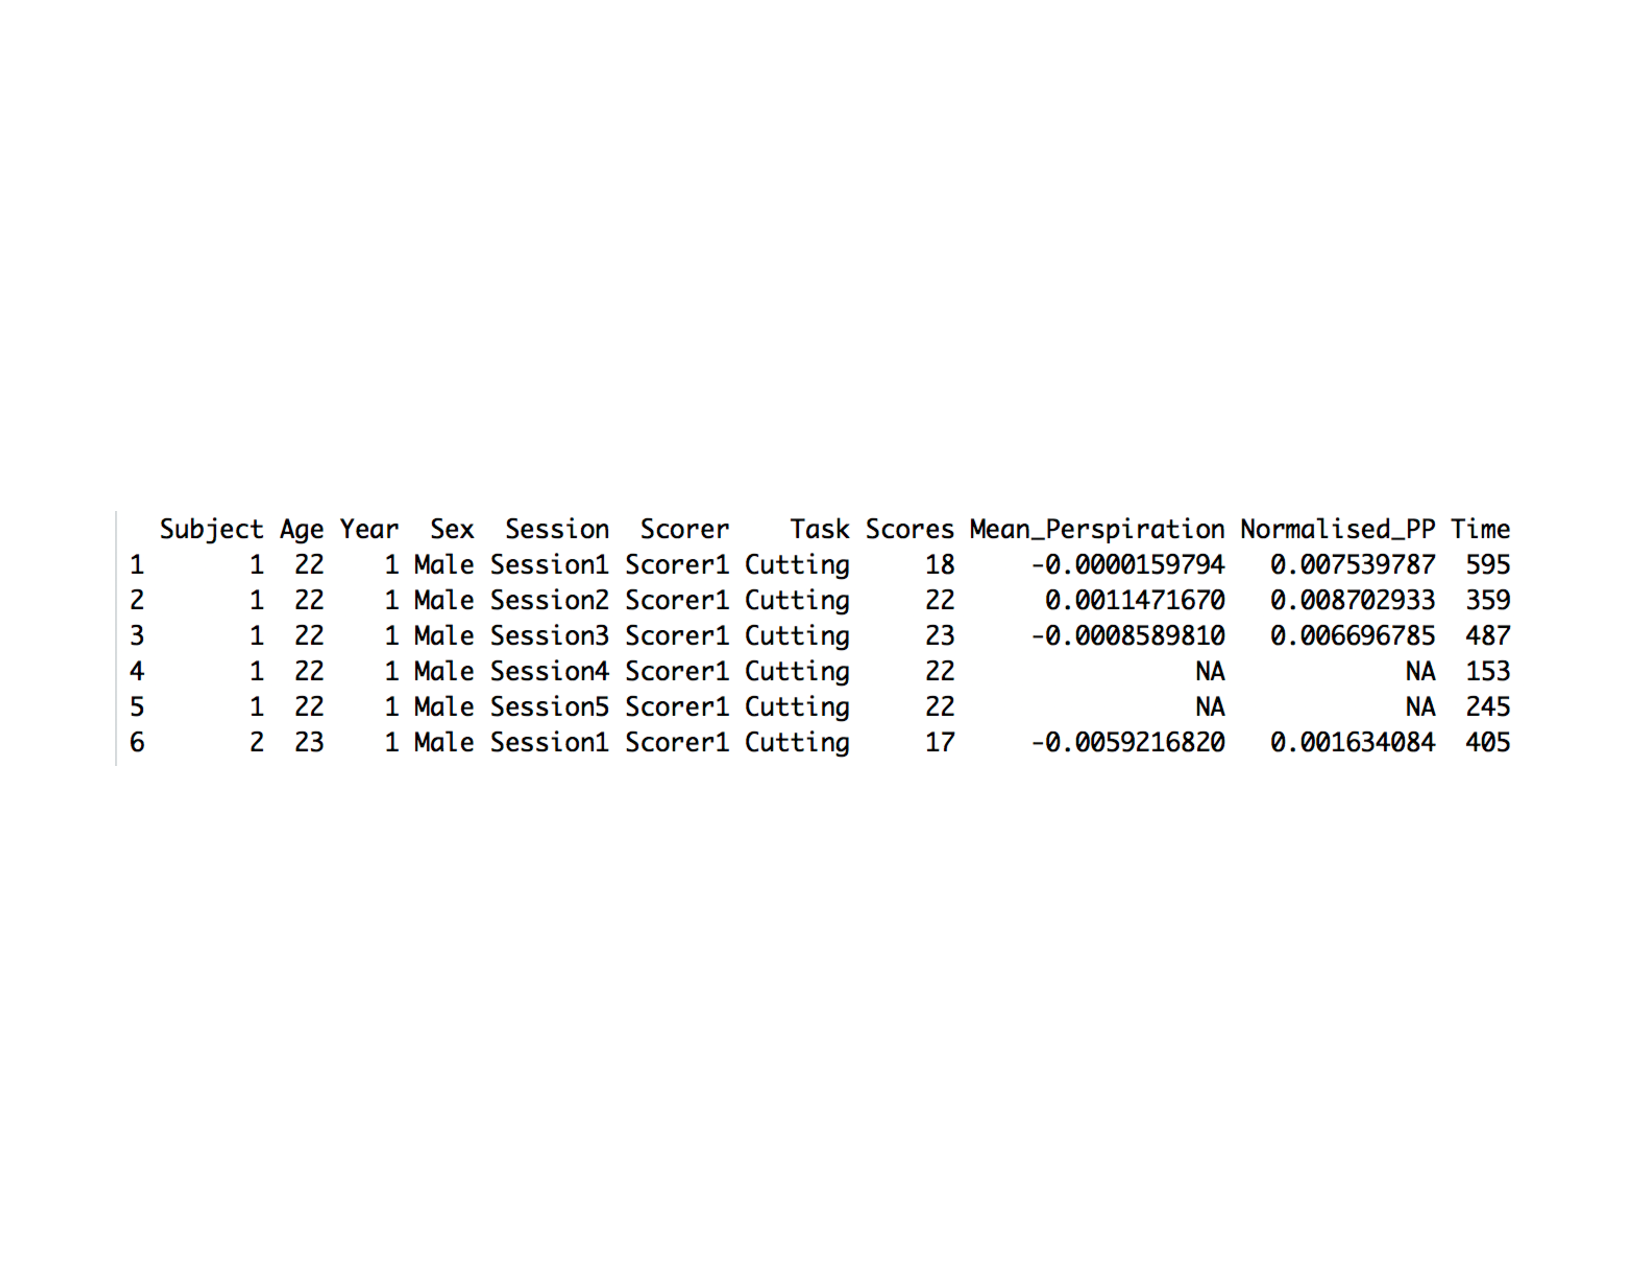
\includegraphics[width=1.1\textwidth]{New_data.pdf}
	\caption{Data Cleaned for Analysis}
\end{figure}
\newpage
\section*{Initial Analysis}
\addcontentsline{toc}{section}{Initial Analysis}
\FloatBarrier
\subsection*{Correlation Matrix}
With the modified data, we not try to understand the correlation between the values. Highly correlated values can be redundant and we can eliminate that in our classification. When taken correlation between all numeric columns of data , we get the following result, where\\
P-stands for the probable value\\
n stands for number of observations \\
r is the correlation value which can range from -1 to 1.\\
From the data we understand that Age and Year are positively correlated with a r value of 0.83 stating that, with increase in age , year increases.There is no association between sessions and Age, Year and Tai scores. All other attributes are neither highly positively or negatively correlated, i.e each correlation value is neither near to -1 or +1 which gives us a huge scope to perform analysis and interpret results\\
\begin{figure}[!htb]
	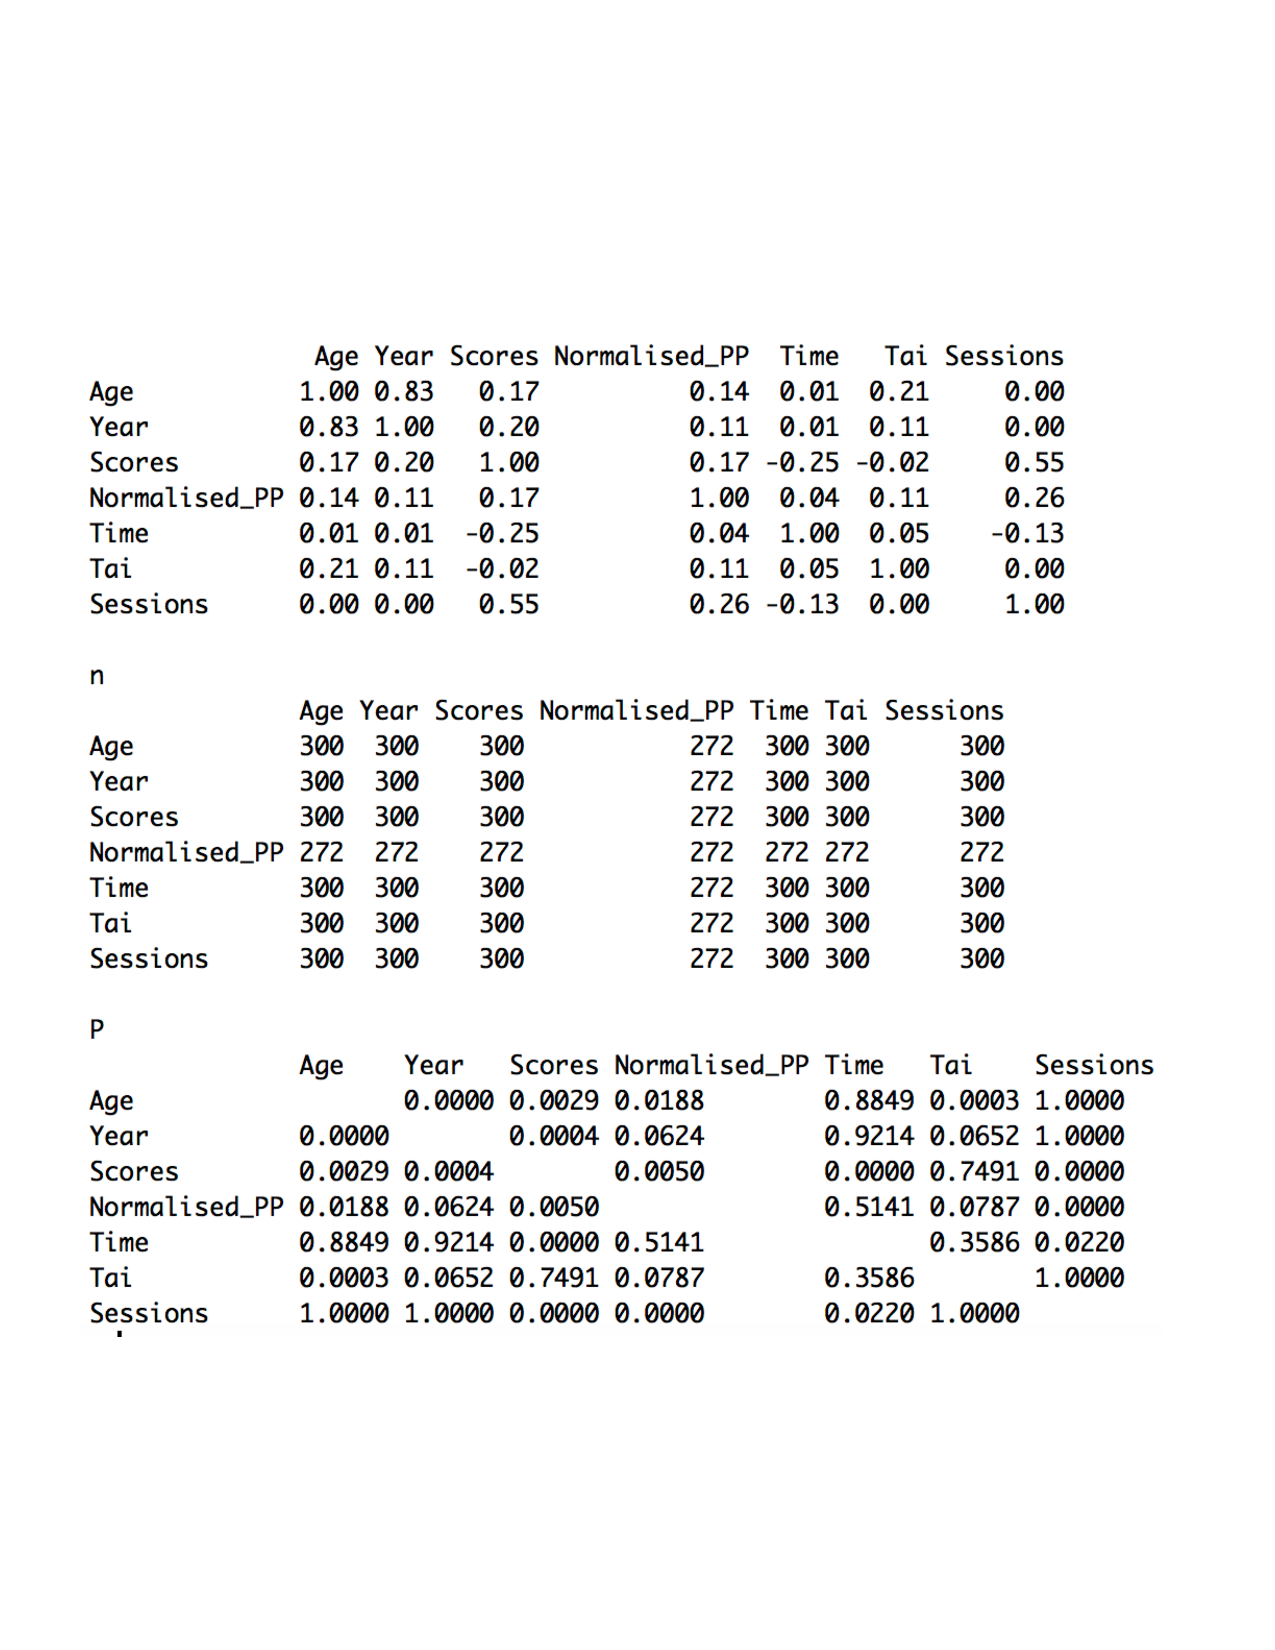
\includegraphics[width=0.9\textwidth]{Correlation_Data.pdf}
	\caption{Correlation Matrix}
\end{figure}
\FloatBarrier
\subsection*{Analysis of Mean Perspiration Based on Subject}
We bar plot the mean perspiration (stress signal)values of all the subjects and of each task.We observe that subjects experienced more stress during the Suturing Task and Subject7 has displayed high level of stress.\\
\begin{figure}[!htb]
	\centering
	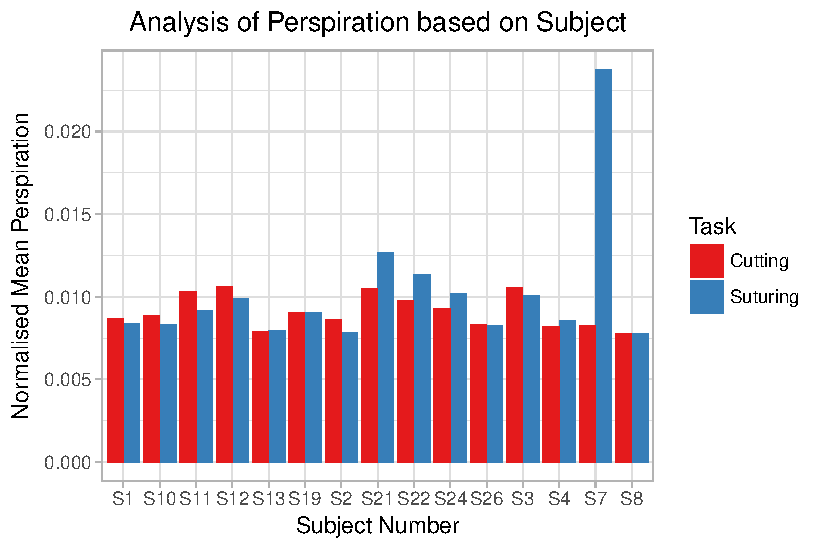
\includegraphics[width=0.6\textwidth]{SubjectVsPP.pdf}
	\caption{Accuracy of Mean Perspiration of all subjects}
	\centering
\end{figure}
\newpage
\FloatBarrier
\section*{Quality Control}
\addcontentsline{toc}{section}{Quality Control}
\FloatBarrier
\subsection*{1.Biographic Data}
\addcontentsline{toc}{subsection}{Biographic Data}
We draw a bar plot to see how gender defines data and histogram to see whether age has any effect on the data.\\
\begin{figure}[!htb]
	\begin{minipage}[c]{0.5\linewidth}
	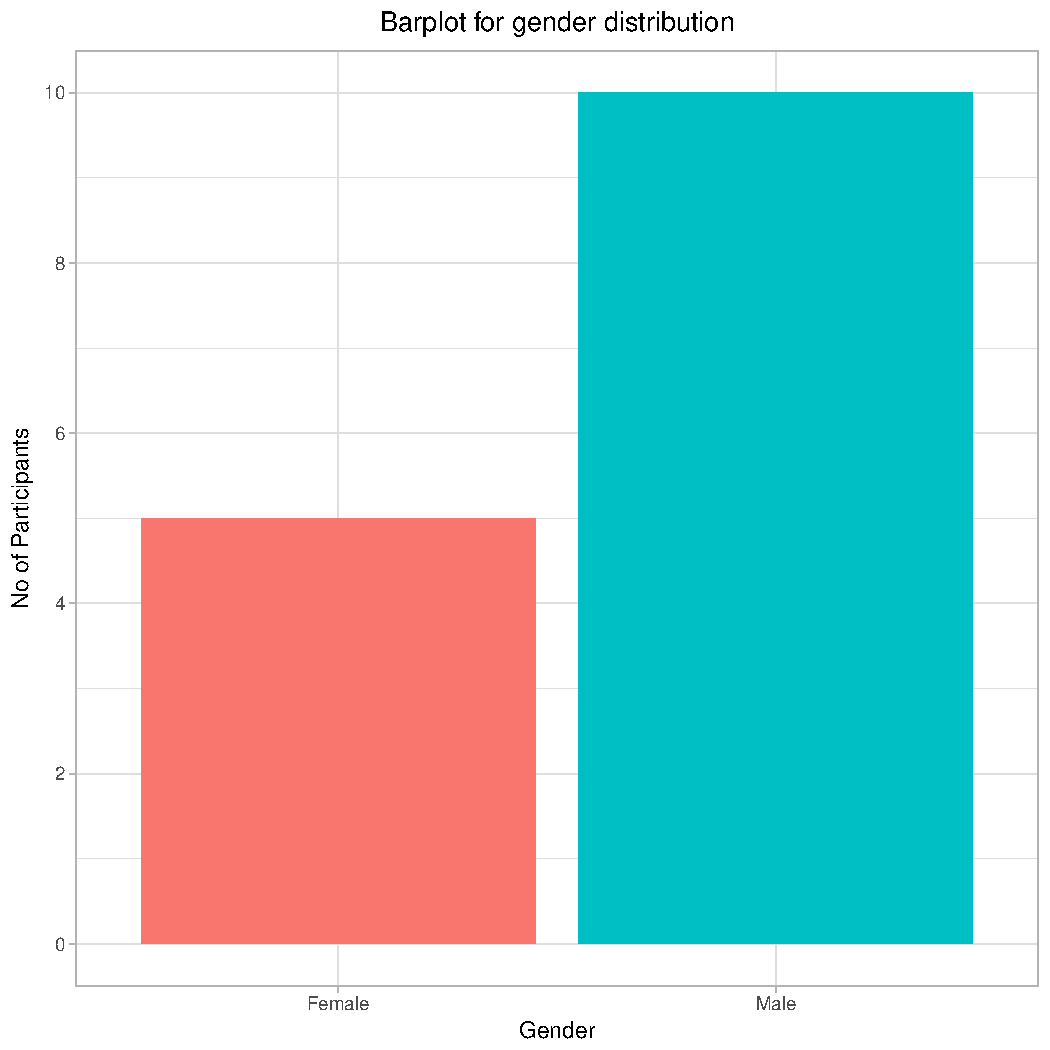
\includegraphics[width=\linewidth]{1_gender.pdf}
	\caption{Barplot of Gender Distribution}
	\end{minipage}
	\hfill
	\begin{minipage}[c]{0.5\linewidth}
	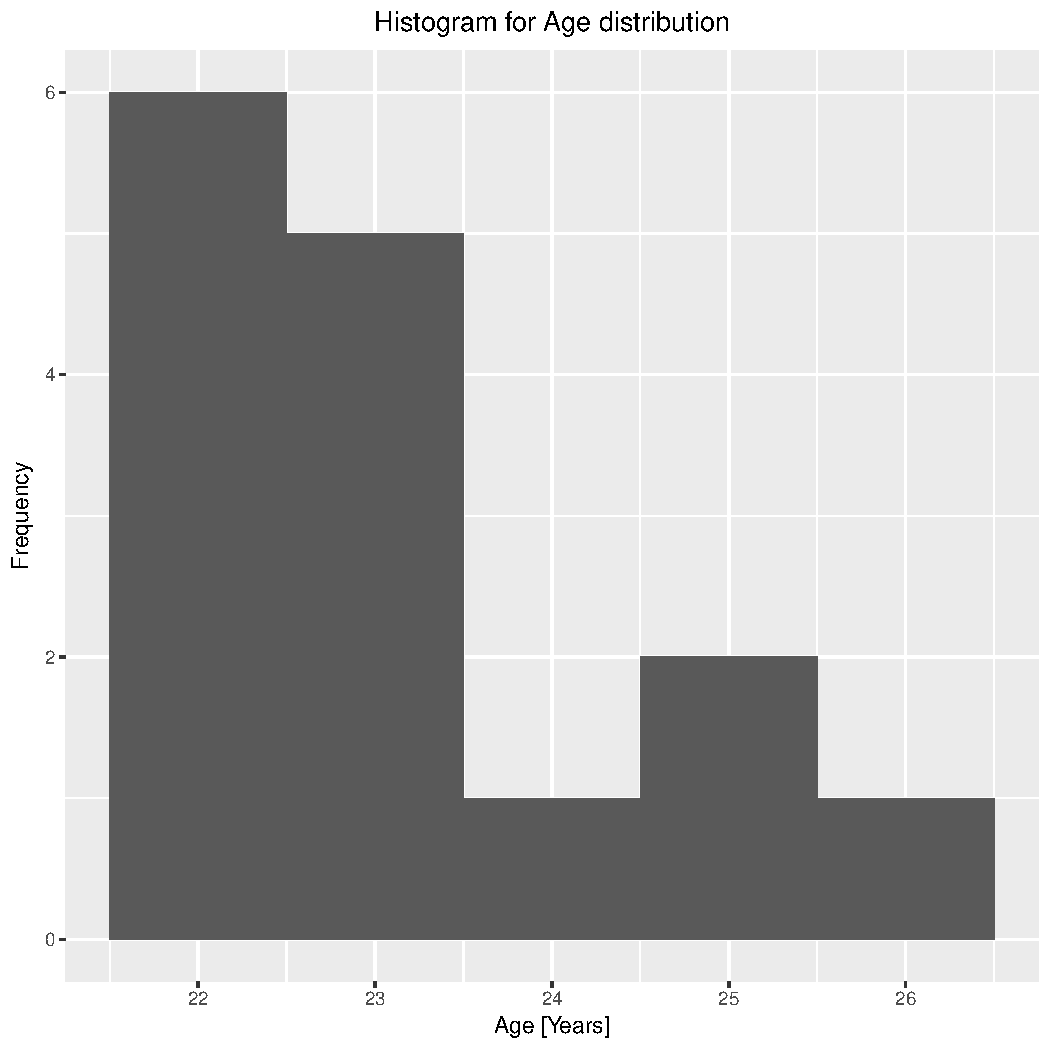
\includegraphics[width=\linewidth]{1_age.pdf}
	\caption{Histogram of age distribution}
	\end{minipage}
\end{figure}
\FloatBarrier
\subsection*{2.Trait Psychometric Data}
\addcontentsline{toc}{subsection}{Trait Psychometric Data}
We draw the histogram for Trait Anxiety Inventory(TAI) scores\\
\begin{figure}[!htb]
	\centering
	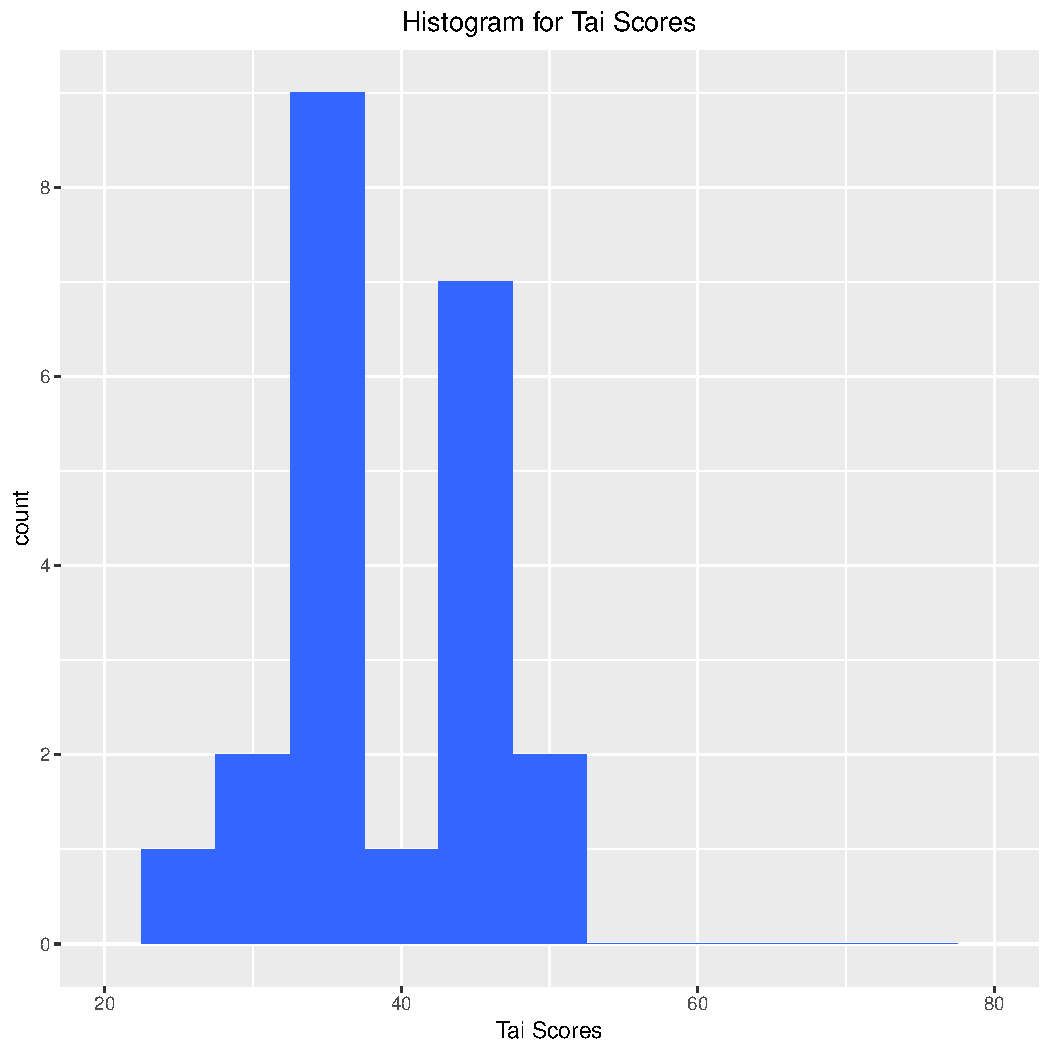
\includegraphics[width=0.5\textwidth]{tai_plot.pdf}
	\caption{Histogram of Tai Scores}
	\centering
\end{figure}
\FloatBarrier
\subsection*{3.State Psychometric Data}
\addcontentsline{toc}{subsection}{State Psychometric Data}
For each subject draw the bar plots for all the NASA-TLX subscales per task. This will give two figures per subject per subscale, one for suturing and one for cutting, where the evolution of the scores from the initial to the final session will be evident. \\
\begin{figure}[!htb]
	\begin{minipage}[c]{0.5\linewidth}
	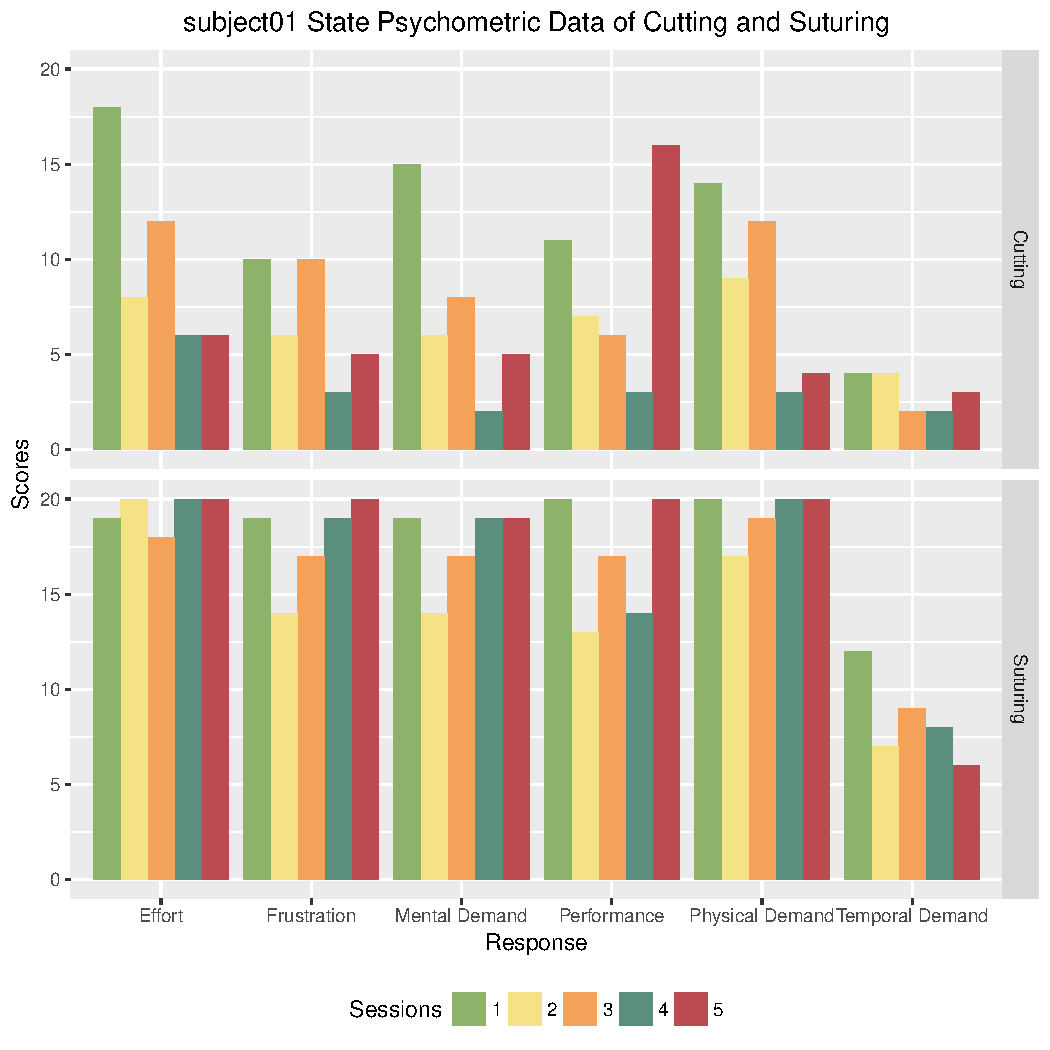
\includegraphics[width=\linewidth]{subject01_State_Psychometric_Data_of_Cutting_and_Suturing.pdf}
	\caption{Subject 1 }
	\end{minipage}
	\hfill
	\begin{minipage}[c]{0.5\linewidth}
	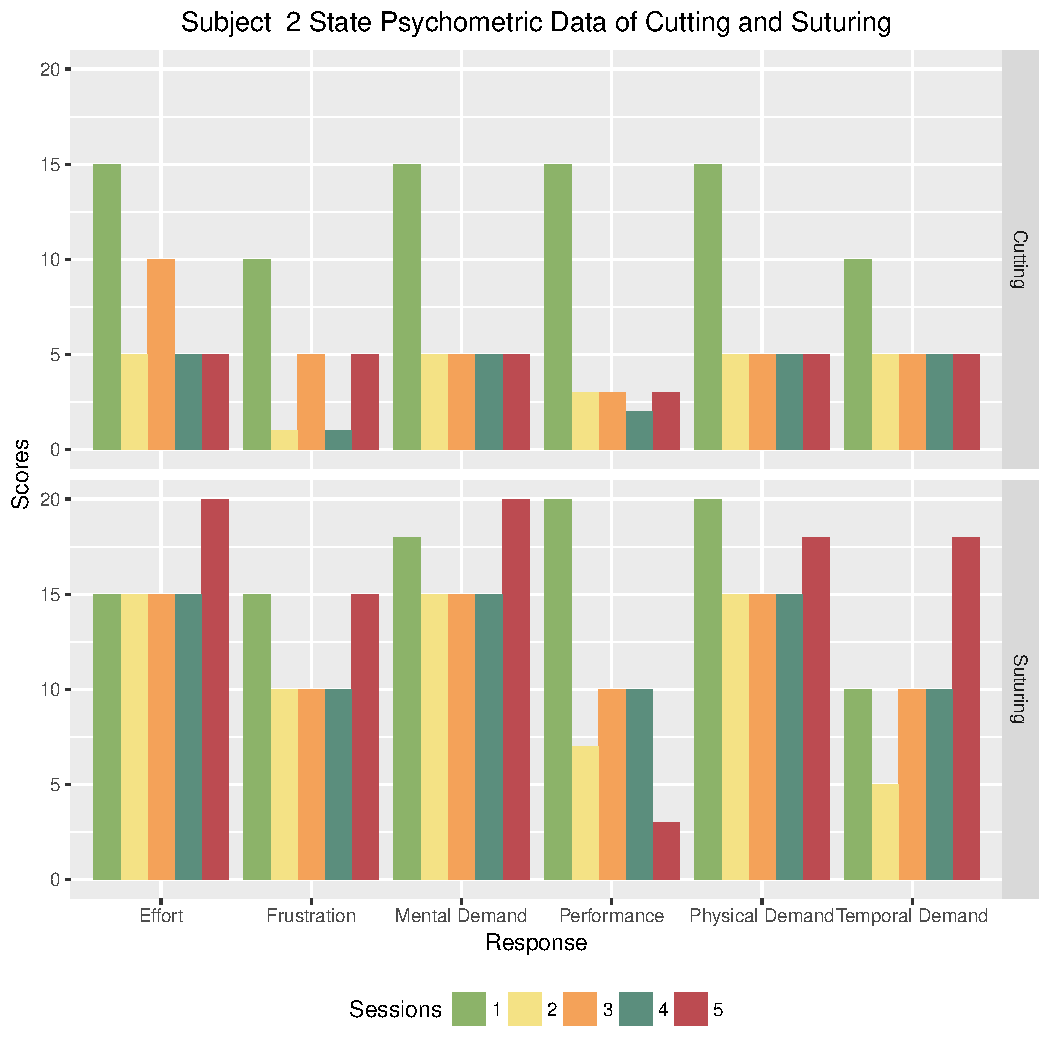
\includegraphics[width=\linewidth]{subject02_State_Psychometric_Data_of_Cutting_and_Suturing.pdf}
	\caption{Subject 2}
	\end{minipage}
\end{figure}
\FloatBarrier
\subsection*{4.Perinasal Perspiration (Stress) Signal Data}
\addcontentsline{toc}{subsection}{Perinasal Perspiration (Stress) Signal Data}
For each session of each subject  we draw the perspiration values using black for baseline, green for cutting, and red for suturing. 
\begin{figure}[!htb]
	\begin{minipage}[c]{0.5\linewidth}
	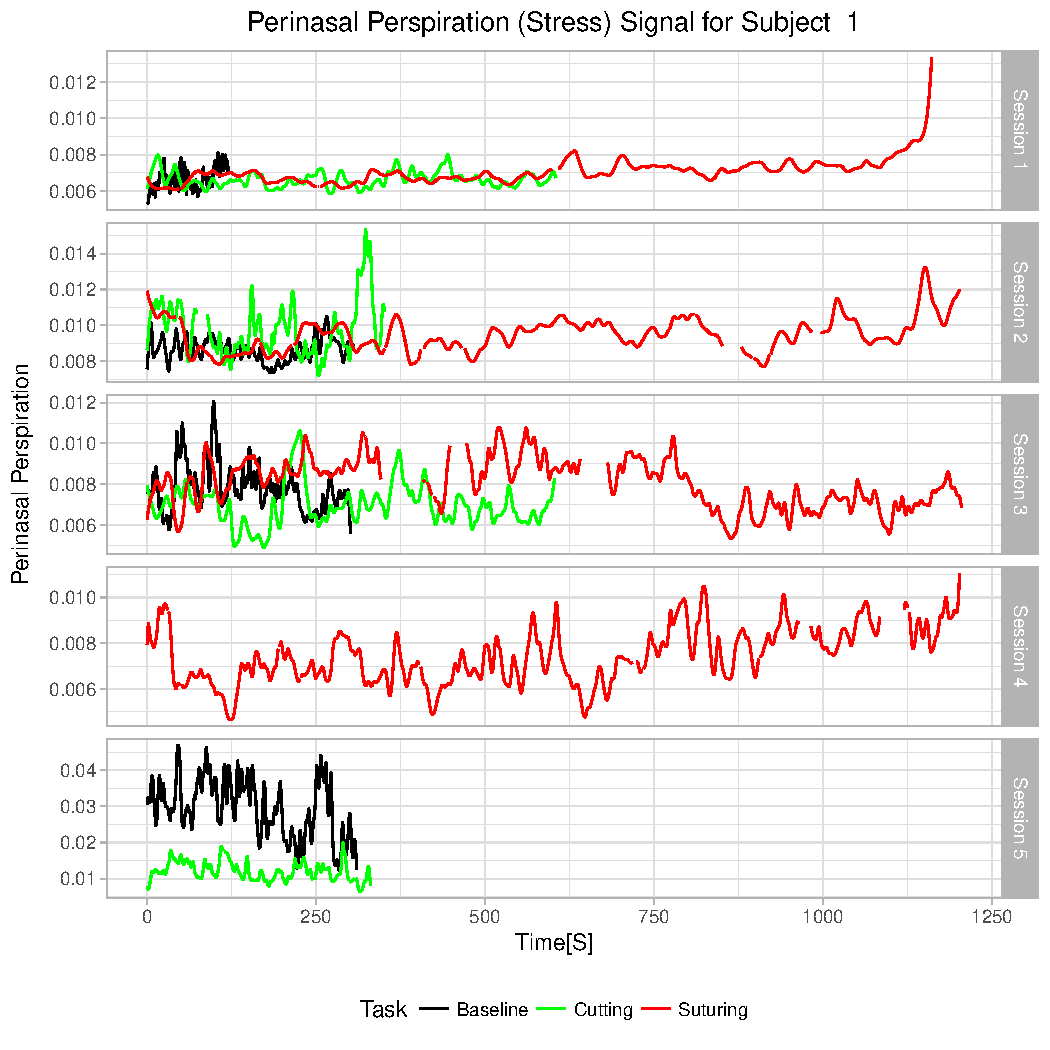
\includegraphics[width=\linewidth]{01_Perinasal_Perspiration.pdf}
	\caption{Subject 1 }
	\end{minipage}
	\hfill
	\begin{minipage}[c]{0.5\linewidth}
	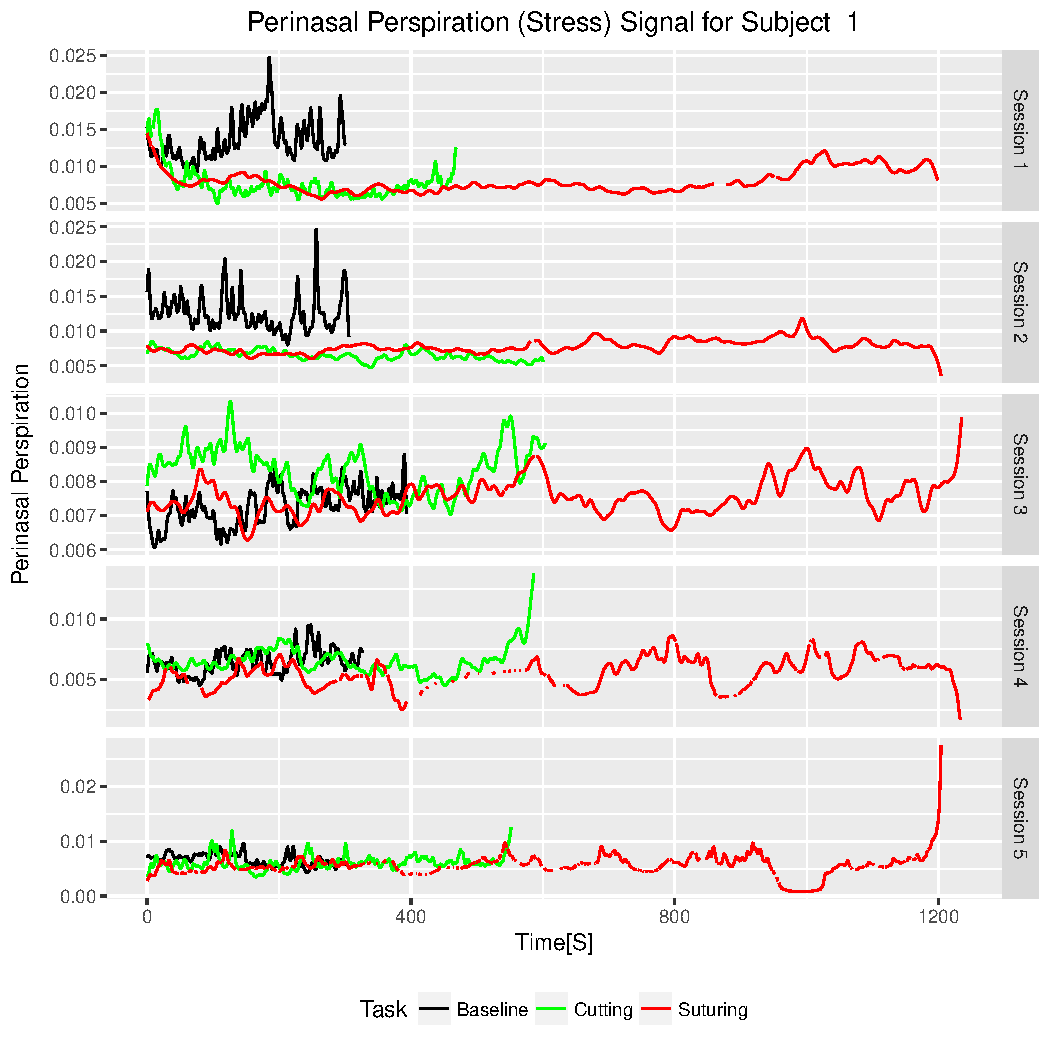
\includegraphics[width=\linewidth]{02_Perinasal_Perspiration.pdf}
	\caption{Subject 2}
	\end{minipage}
\end{figure}
\FloatBarrier
\subsection*{5.Performance Data}
\addcontentsline{toc}{subsection}{Performance Data}
We draw the accuracy and time bar plots of each subject for each session and each task.\\
\begin{figure}[!htb]
	\centering
	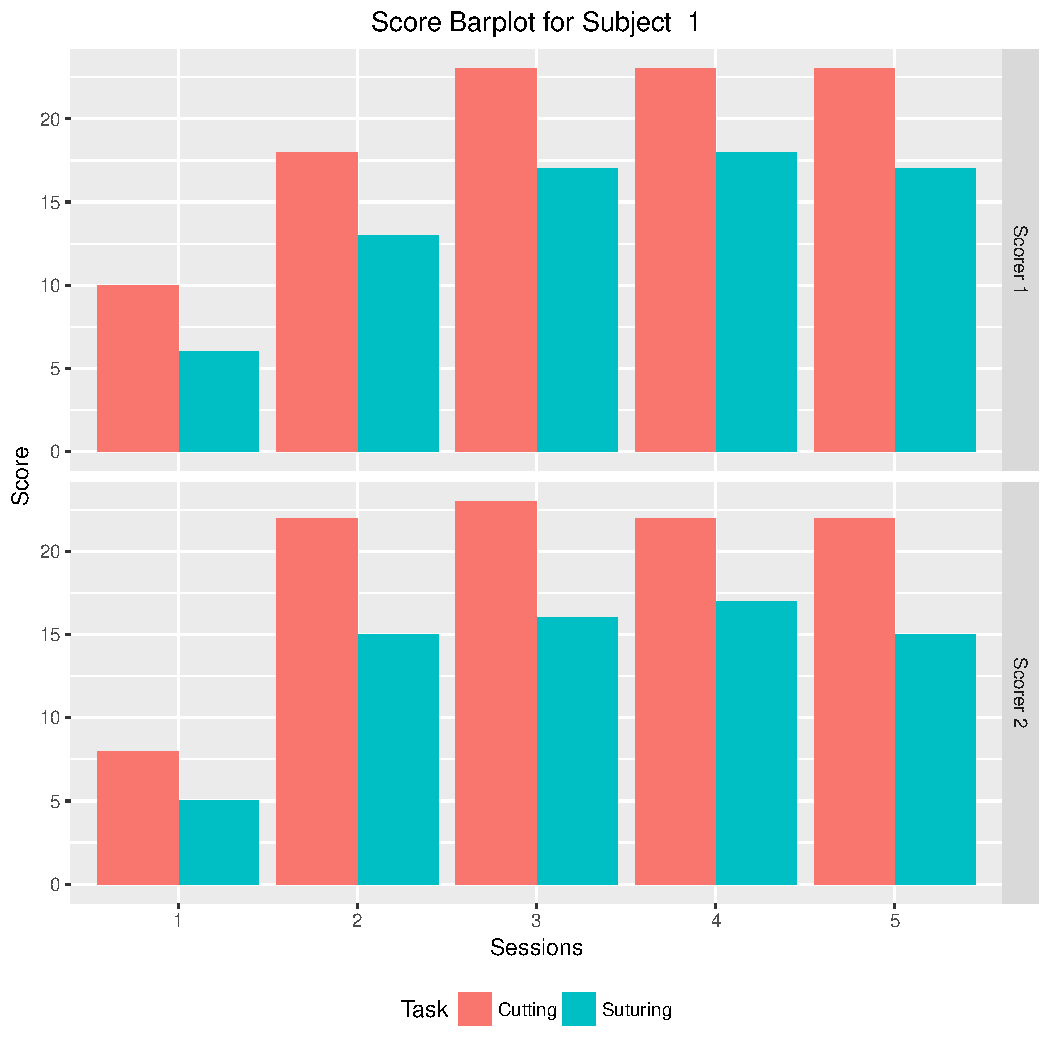
\includegraphics[width=0.5\textwidth]{1_Score_barplot.pdf}
	\caption{Subject 1 Score Barplot}
	\centering
\end{figure}
\\
\begin{figure}[!htb]
	\centering
	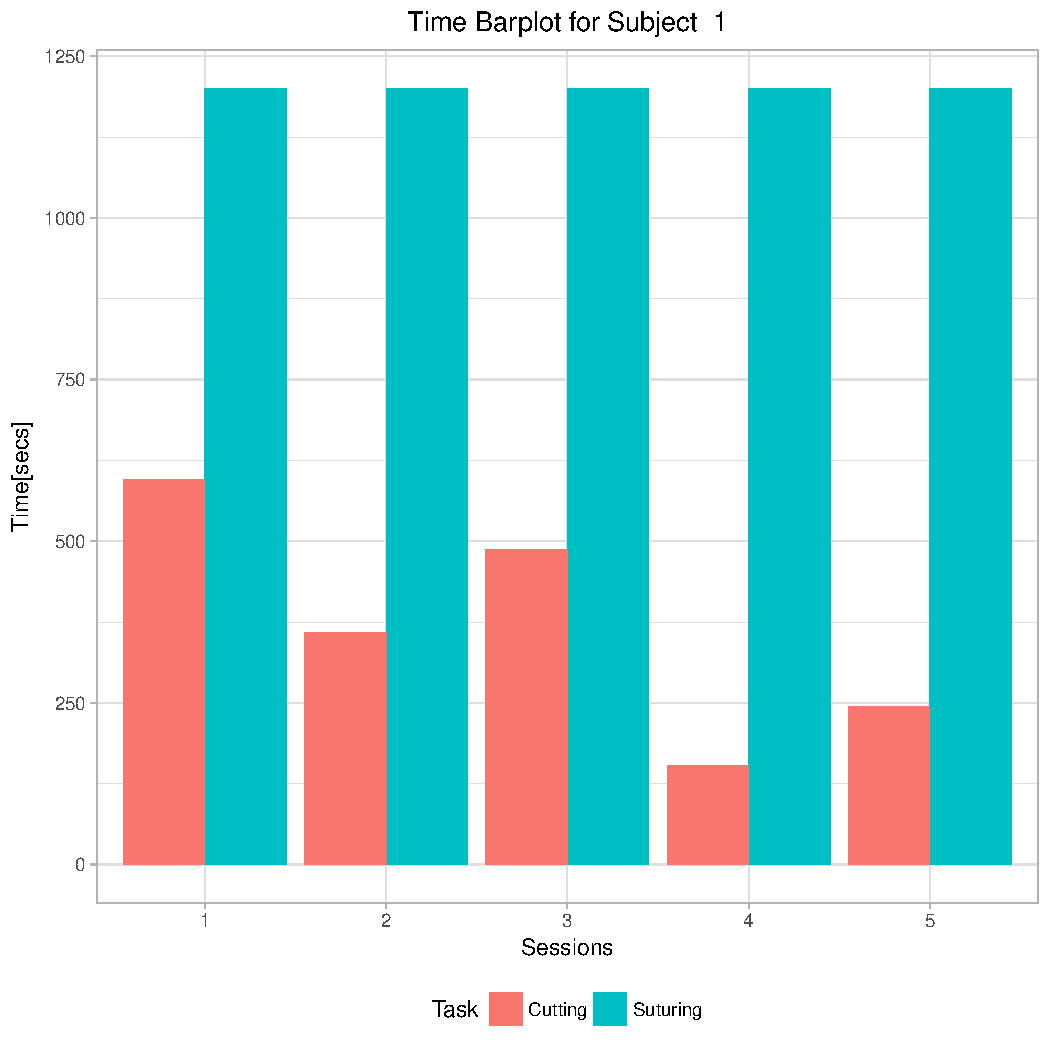
\includegraphics[width=0.5\textwidth]{1_Time_barplot.pdf}
	\caption{Subject 1 Time Barplot}
	\centering
\end{figure}\\
\section*{Hypothesis Testing}
We now perform various tests to determine significance of any factor on the other and make inferences about the performance of the subjects in tasks.\\
\addcontentsline{toc}{section}{Hypothesis Testing}
\subsection*{1. Analysis of effect of each attribute on Score}
\addcontentsline{toc}{subsection}{Analysis of effect of each attribute on Score}
\textbf{Hypothesis}:\\
Null Hypothesis : $H_0$ =  The score obtained does not depend on the demographics of the subject , session , age , year , sex and perspiration.\\
Alternate Hypothesis : $H_1$ =  The score obtained  depends on the demographics of the subject , session , age , year , sex and perspiration.\\
\\
\textbf{Approach:Linear Modelling}:\\
Linear modeling gives the relationship between the dependent and independent variables. 
In our data set we are finding the hypothesis between each attribute such as Age, sex, year and mean perspiration with the scores of scorer.\\
\begin{figure}[!htb]
	\centering
	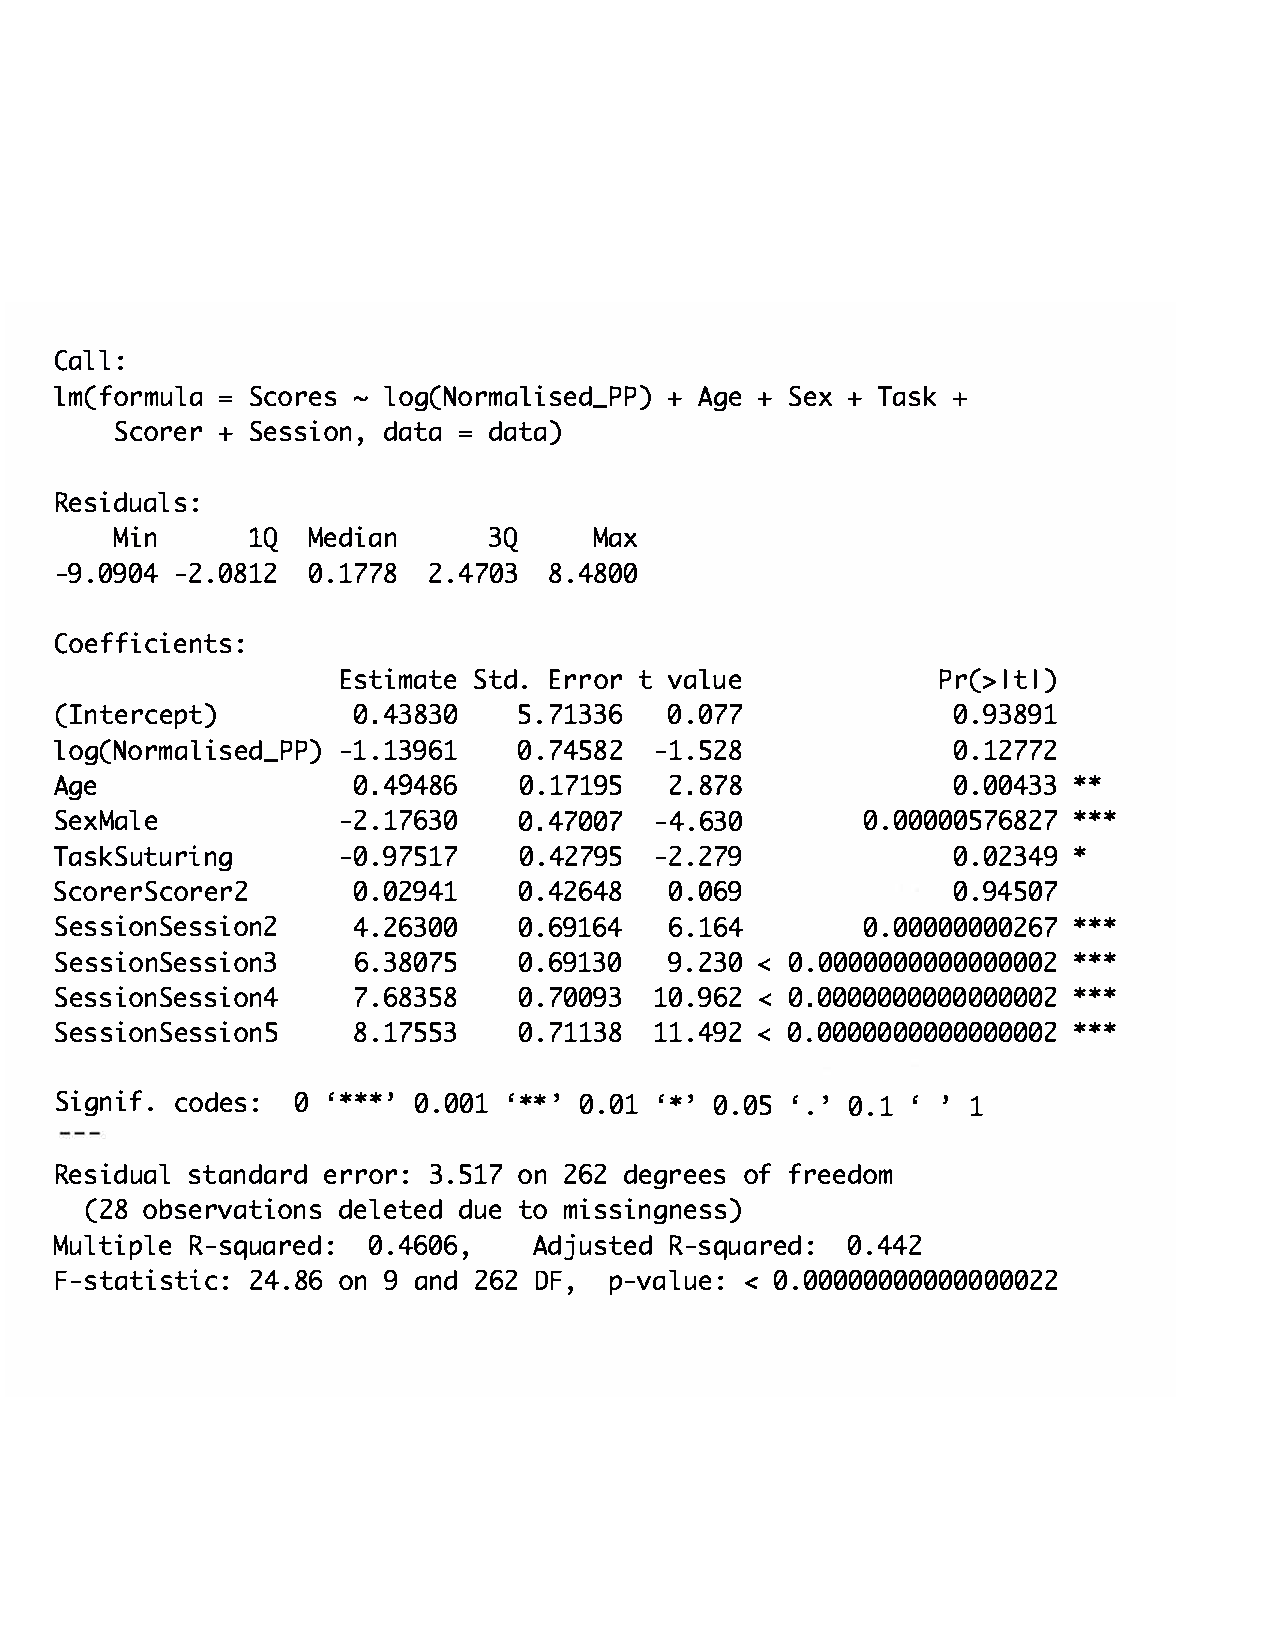
\includegraphics[width=0.8\textwidth]{ScoreSummary.pdf}
	\caption{Linear model of score vs all other attributes}
	\centering
\end{figure}
When we performed the linear model and analyzed the results, we observe that the pvalue is way less than 0.05, thus rejecting the null hypothesis. We also observe that the Score is highly Significant on Sex and Sessions.\\
\\
\begin{figure}[!htb]
	\begin{minipage}[c]{0.5\linewidth}
	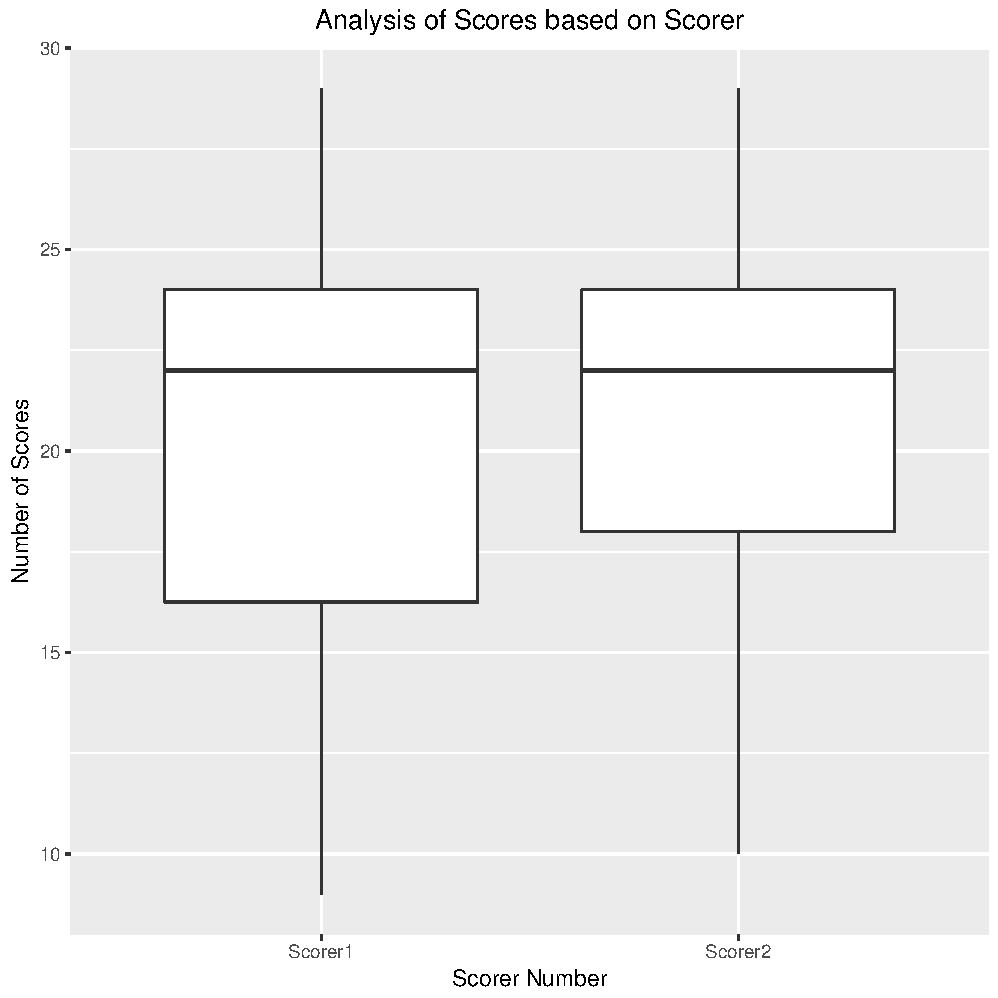
\includegraphics[width=\linewidth]{ScorerVsScore.pdf}
	\caption{Analysis of Scores based on Score }
	\end{minipage}
	\hfill
	\begin{minipage}[c]{0.5\linewidth}
	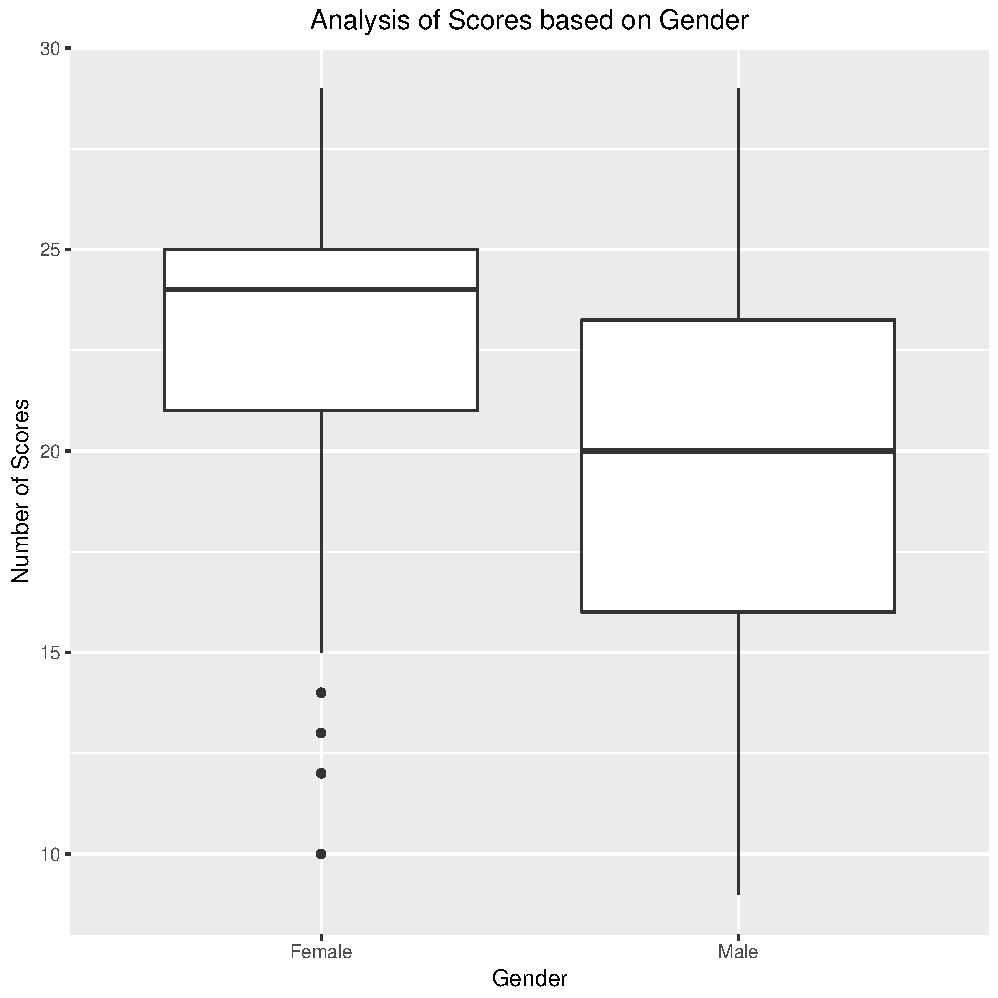
\includegraphics[width=\linewidth]{GenderVsScore.pdf}
	\caption{Analysis of Scores based on Gender}
	\end{minipage}
\end{figure}
\begin{figure}[!htb]
	\begin{minipage}[c]{0.5\linewidth}
	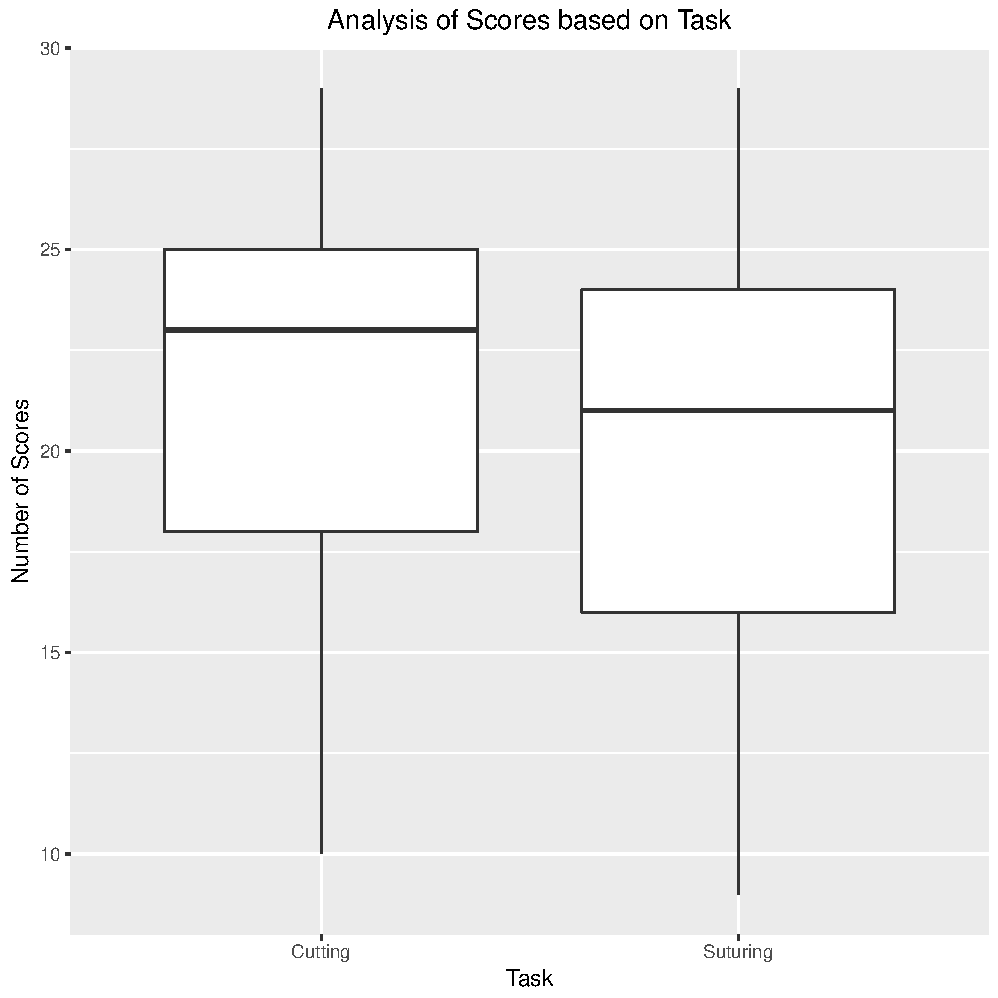
\includegraphics[width=\linewidth]{TaskVsScore.pdf}
	\caption{Analysis of Scores based on Task}
	\end{minipage}
	\hfill
	\begin{minipage}[c]{0.5\linewidth}
	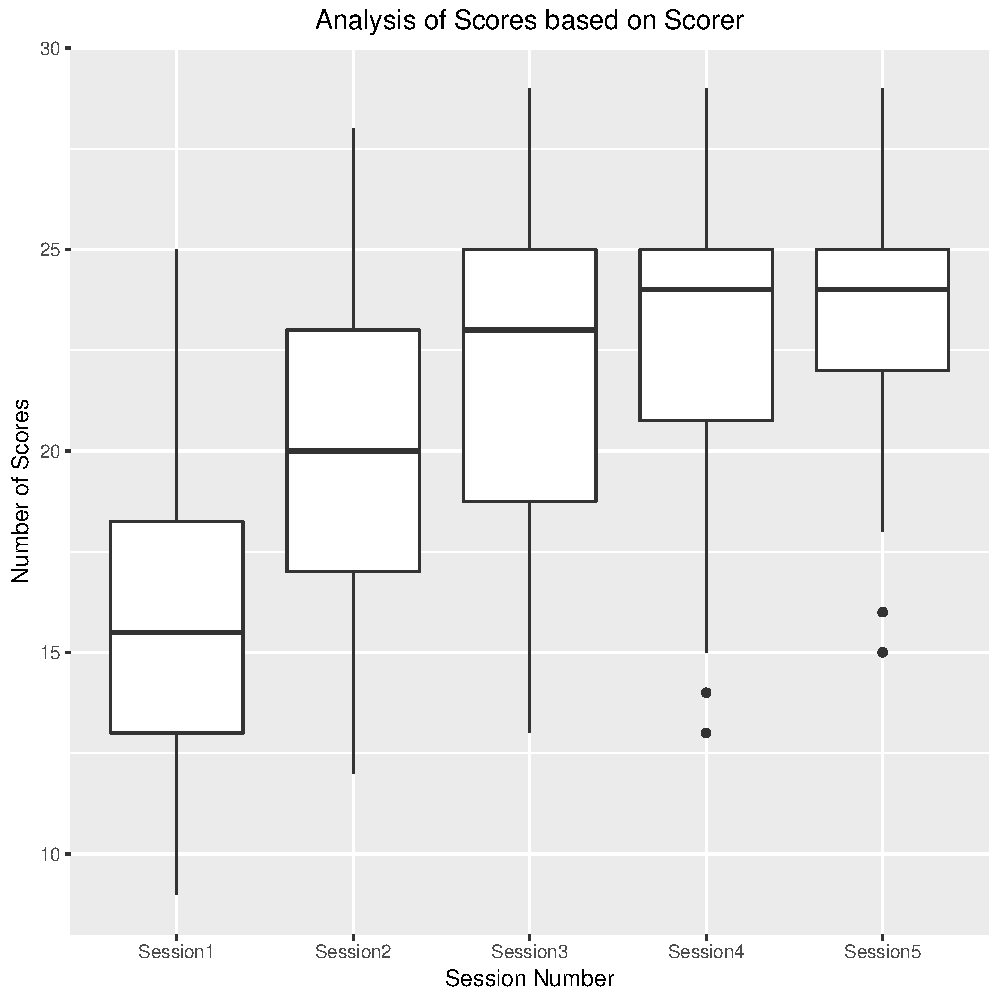
\includegraphics[width=\linewidth]{SessionVsScore.pdf}
	\caption{Analysis of Scores based on Session}
	\end{minipage}
\end{figure}\\
\\
\textbf{Inference}:\\
From the plots and linear model, we infer that the score is highly dependent on Sex, Session number and nearly significant on the Task.\\
\\
\\
\FloatBarrier
\subsection*{2. Analysis of effect of each attribute on Time}
\addcontentsline{toc}{subsection}{Analysis of effect of each attribute on Time}
\textbf{Hypothesis}:\\
Null Hypothesis : $H_0 $=  The time taken to do a task is not dependent of age, session, sex, Perspiration.\\
Alternate Hypothesis : $H_1$ =  he time taken to do a task depends on  age, session, sex, Perspiration.\\
\\
\textbf{Approach:Linear Modelling}:\\
Linear modeling gives the relationship between the dependent and independent variables. 
In our data set we are finding the hypothesis between each attribute such as Age, sex,Scorer,Task,Session and mean perspiration with the time taken to do the task.\\
\begin{figure}[!htb]
	\centering
	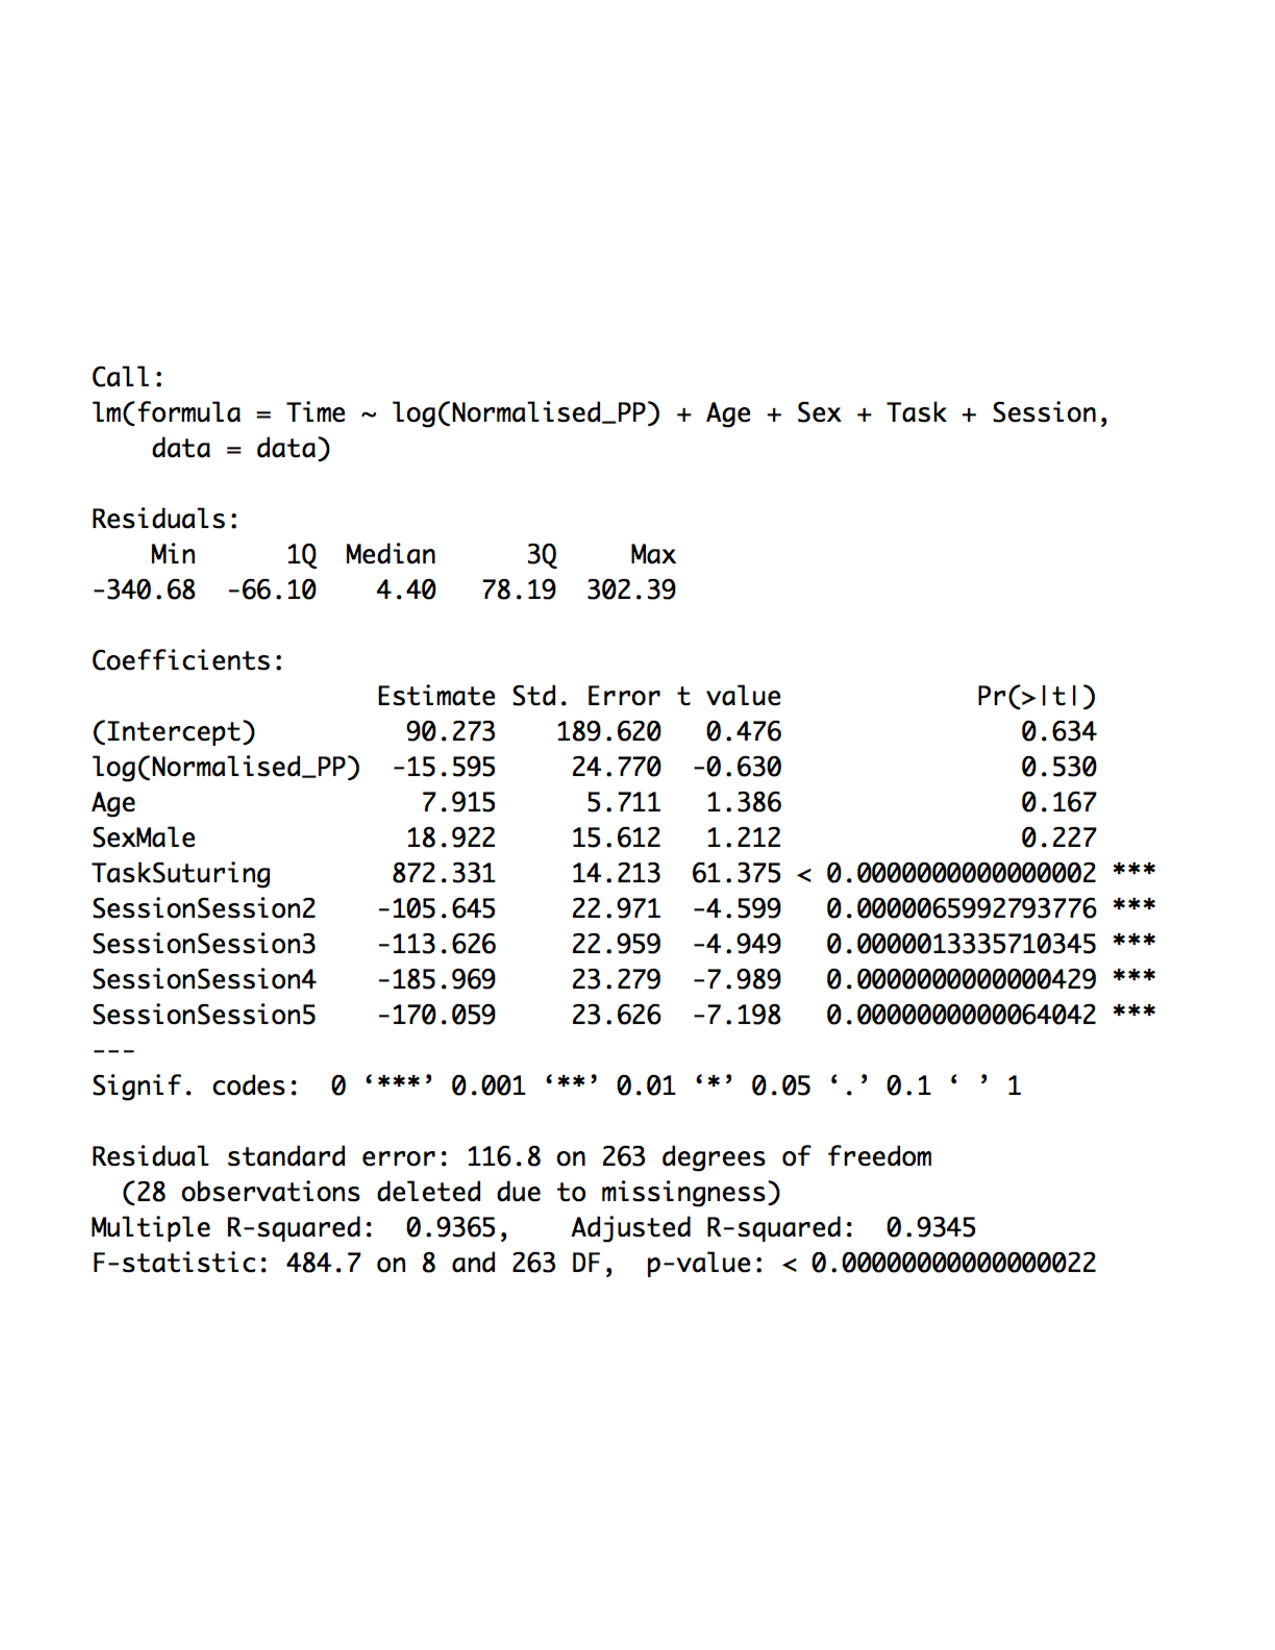
\includegraphics[width=0.8\textwidth]{TimeSummary.pdf}
	\caption{Linear model of Time vs all other attributes}
	\centering
\end{figure}
\\
When we performed the linear model and analyzed the results, we observe that the pvalue is way less than 0.05, thus rejecting the null hypothesis. We also observe that the Time taken is highly Significant on Task and Sessions. \\
\begin{figure}[!htb]
	\begin{minipage}[c]{0.5\linewidth}
	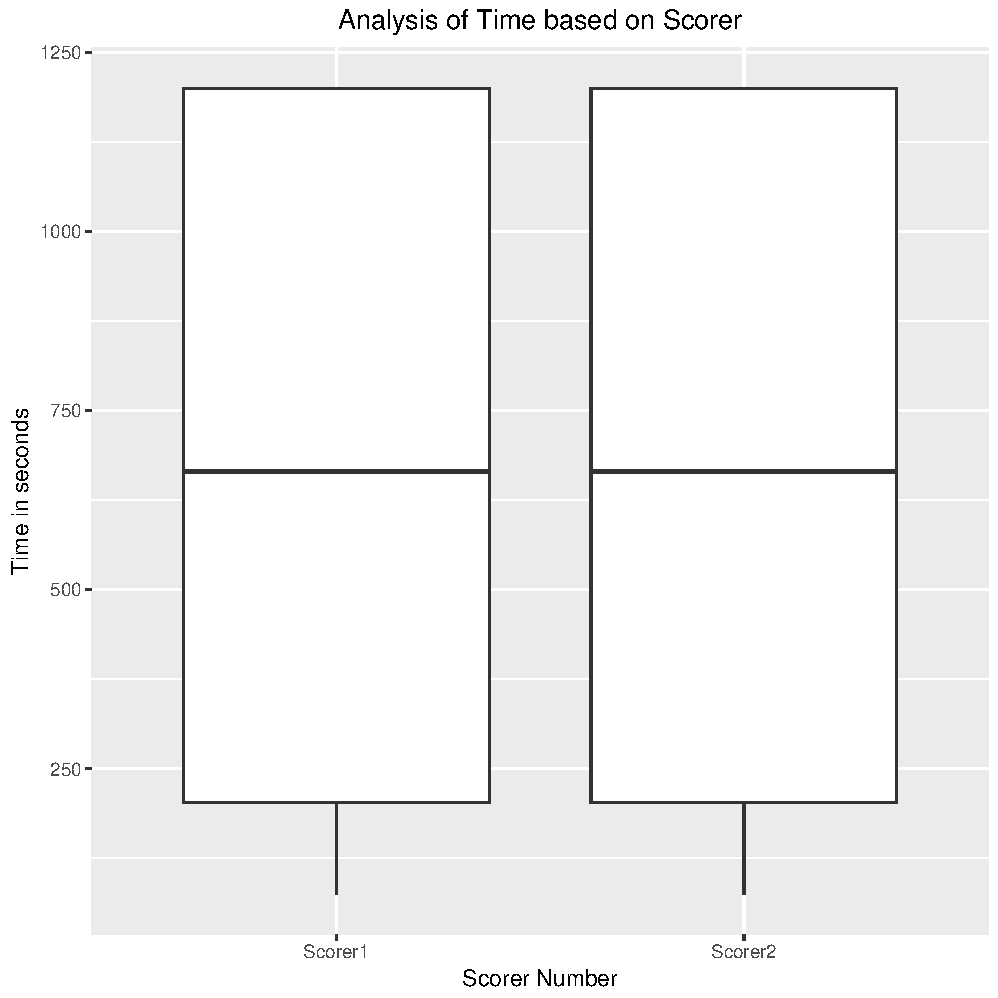
\includegraphics[width=\linewidth]{ScorerVsTime.pdf}
	\caption{Analysis of Time based on Score }
	\end{minipage}
	\hfill
	\begin{minipage}[c]{0.5\linewidth}
	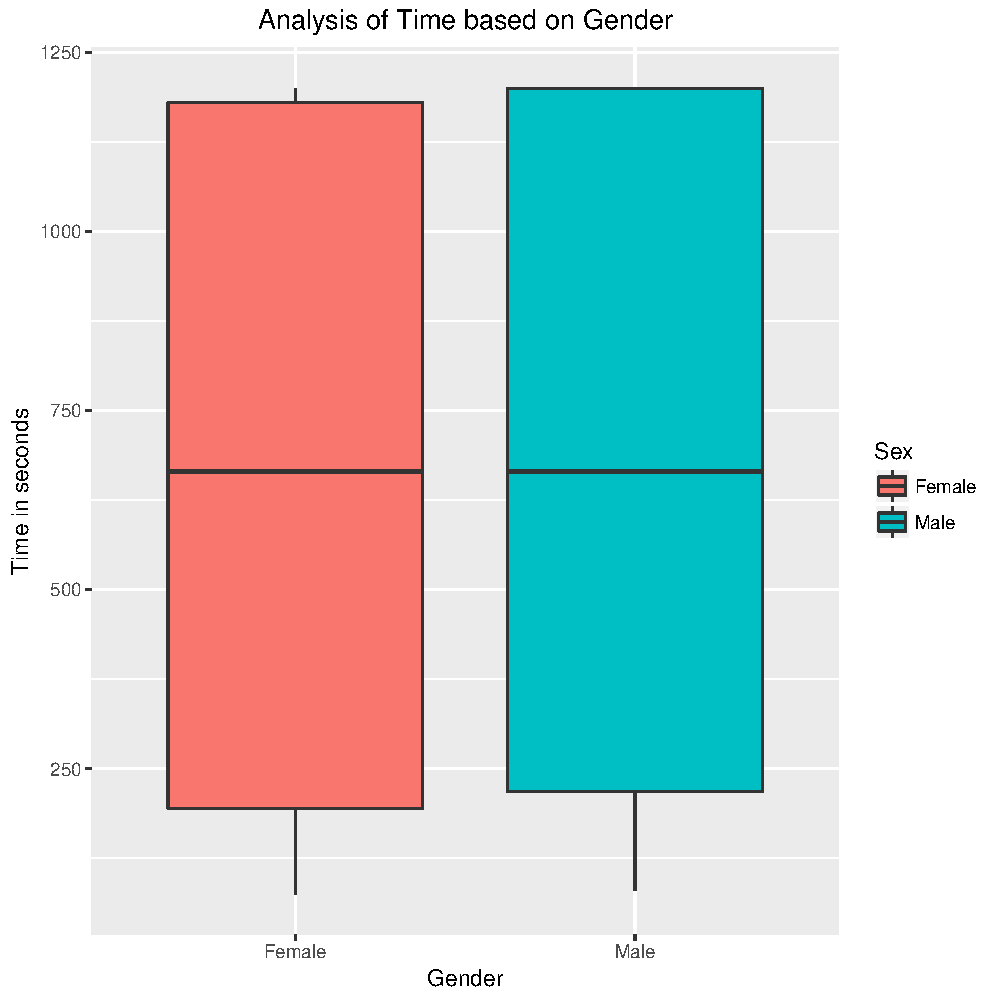
\includegraphics[width=\linewidth]{GenderVsTime.pdf}
	\caption{Analysis of Time based on Gender}
	\end{minipage}
\end{figure}
\begin{figure}[!htb]
	\begin{minipage}[c]{0.5\linewidth}
	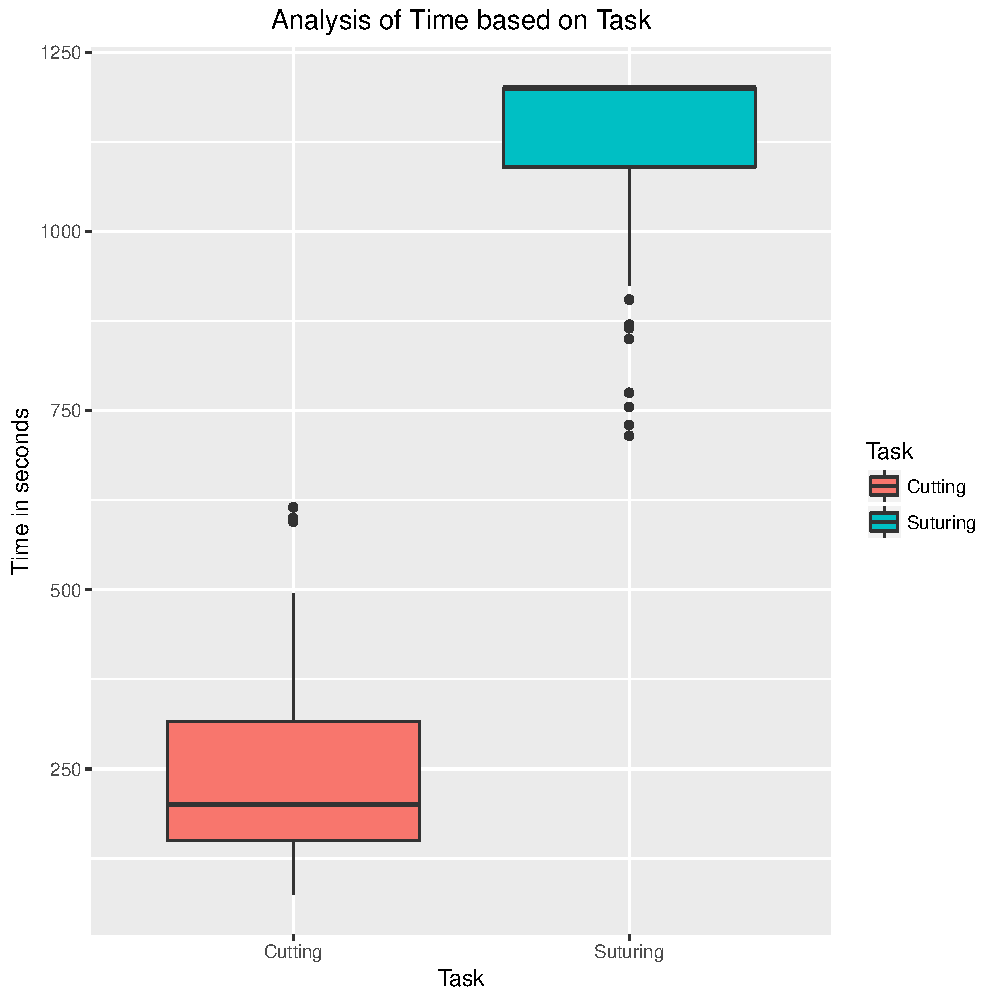
\includegraphics[width=\linewidth]{TaskVsTime.pdf}
	\caption{Analysis of Time based on Task}
	\end{minipage}
	\hfill
	\begin{minipage}[c]{0.5\linewidth}
	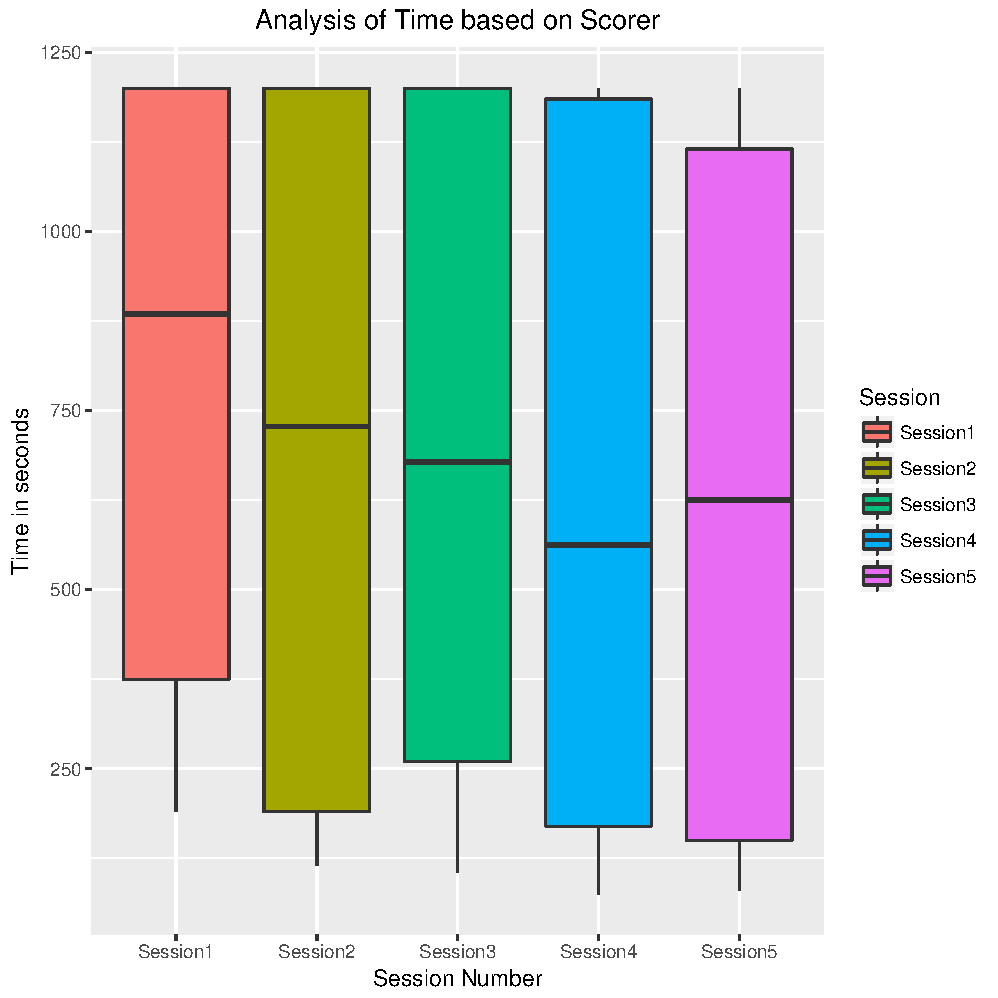
\includegraphics[width=\linewidth]{SessionVsTime.pdf}
	\caption{Analysis of Time based on Session}
	\end{minipage}
\end{figure}\\
\textbf{Inference}:\\
We observe that the means of Time vs Scorer or Gender do not have highly significant difference. Although, Task does have significant difference, we do not take it as a notifiable inference, because the time limits are different for each tasks, with time to complete suturing task being. 20 minutes. Hence, From the summary and the plots we infer that the time taken highly depends on the sessions.\\
\\
\FloatBarrier
\subsection*{3. Performance Analysis of Suturing Task}
\addcontentsline{toc}{subsection}{Performance Analysis of Suturing Task}
We first perform a correlation between number of sutures made and subject, age, time taken scorer, scores and session. We observe that time and number of sutures made are moderately negatively correlated, which indicates that the subjects are performing better. Also, number of sutures made is highly correlated with the scores. The session is moderately positively correlated with Sutures, indicating a positive relationship. \\
\begin{figure}[!htb]
	\centering
	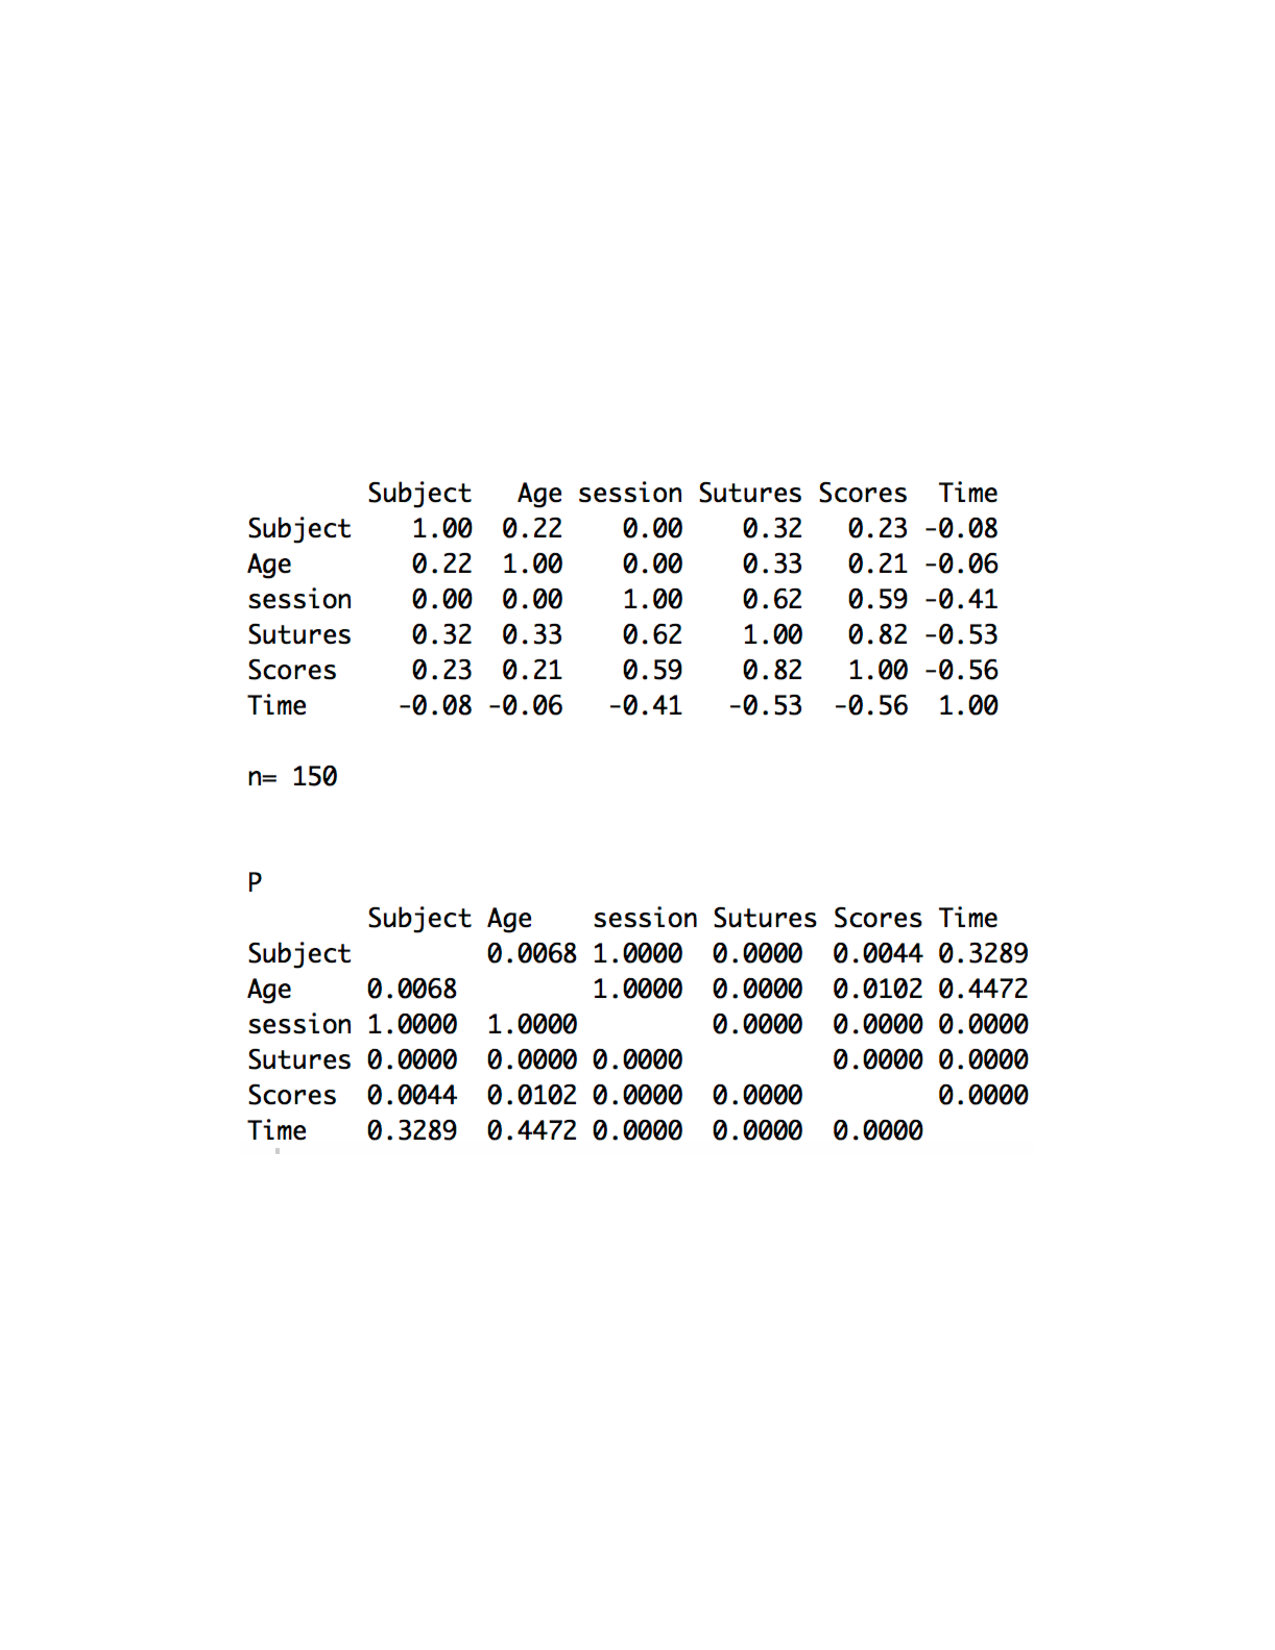
\includegraphics[width=0.7\textwidth]{Corr_Sutures.pdf}
	\caption{Correlation Matrix of Sutures Data}
	\centering
\end{figure}\\
\textbf{Approach:Linear Model}:
\begin{figure}[!htb]
	\begin{minipage}[c]{0.5\linewidth}
	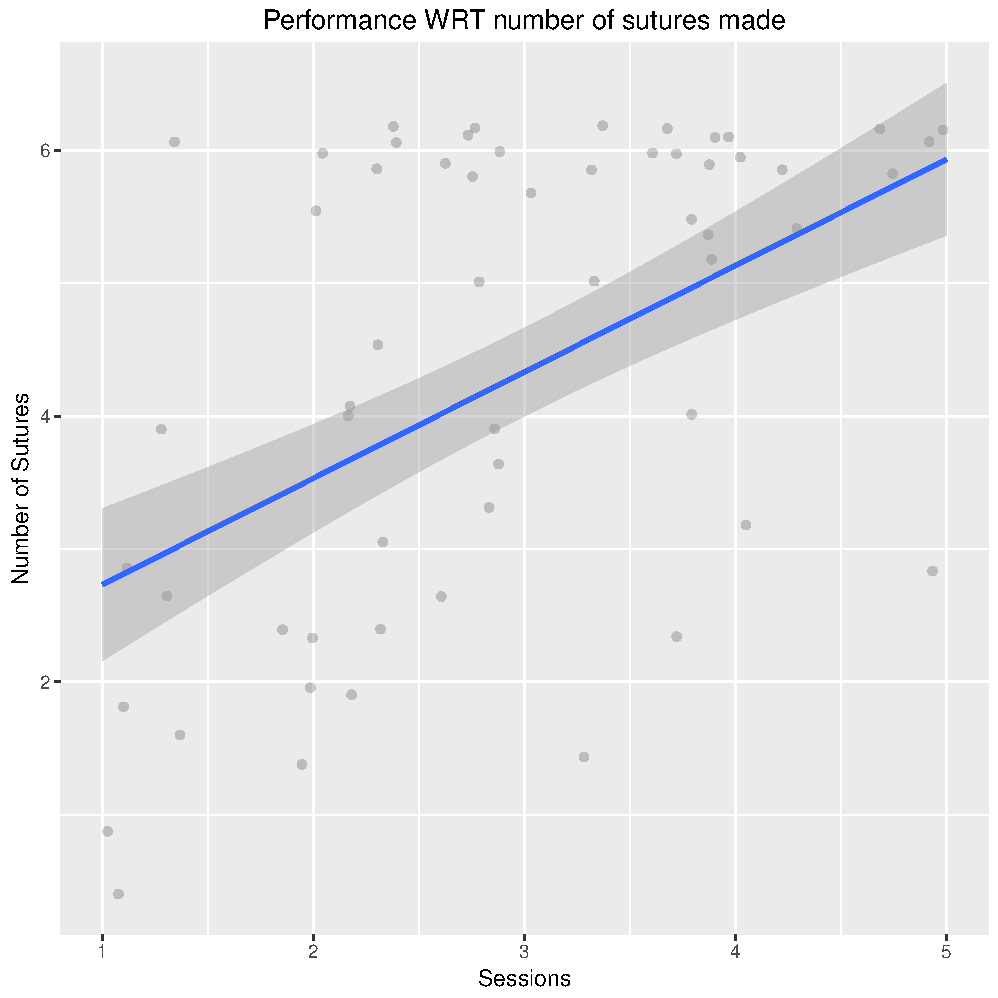
\includegraphics[width=\linewidth]{PerformanceWRTSutures.pdf}
	\caption{Performance WRT number of sutures made}
	\end{minipage}
	\hfill
	\begin{minipage}[c]{0.5\linewidth}
	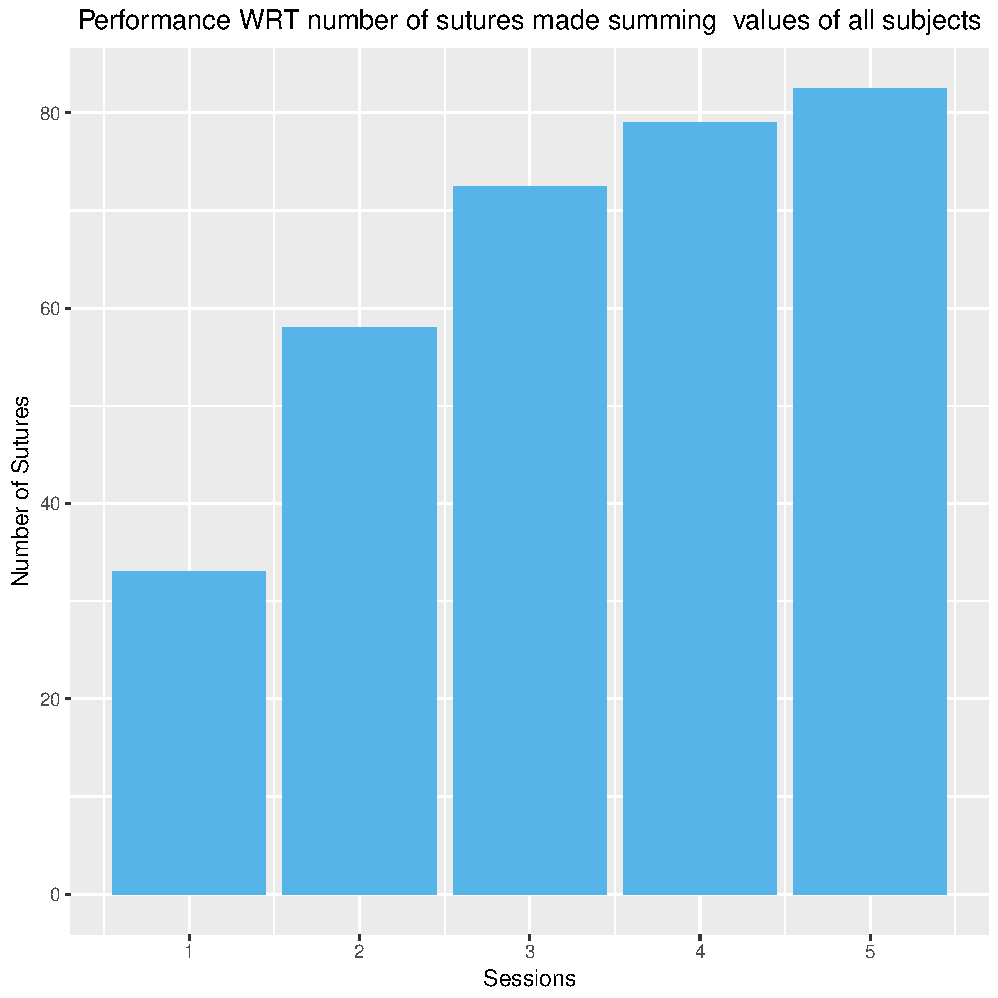
\includegraphics[width=\linewidth]{PerformanceWRTSutures_bar.pdf}
	\caption{Performance WRT number of sutures summed across all subjects}
	\end{minipage}
\end{figure}
\begin{figure}[!htb]
	\centering
	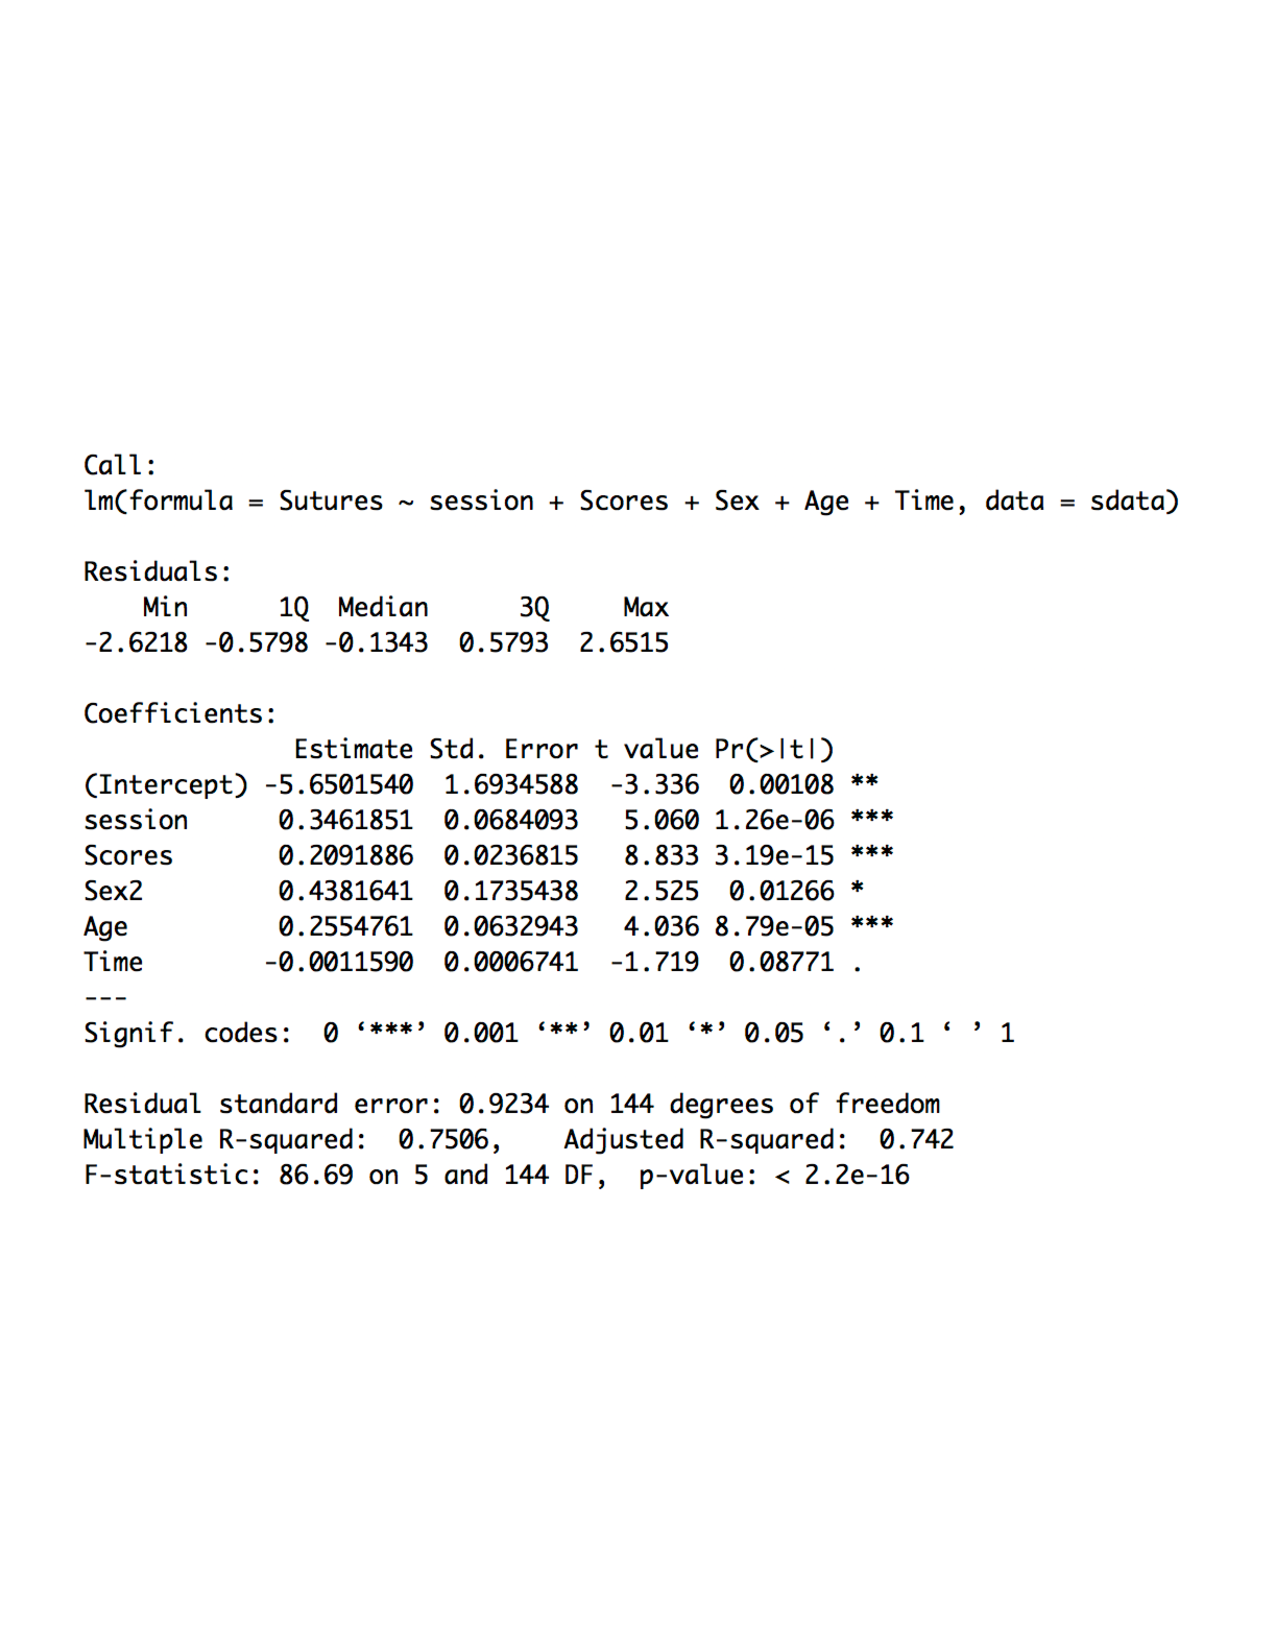
\includegraphics[width=0.7\textwidth]{Sutures_Summary.pdf}
	\caption{Analysis of Linear Model}
	\centering
\end{figure}\\
\begin{figure}[!htb]
	\centering
	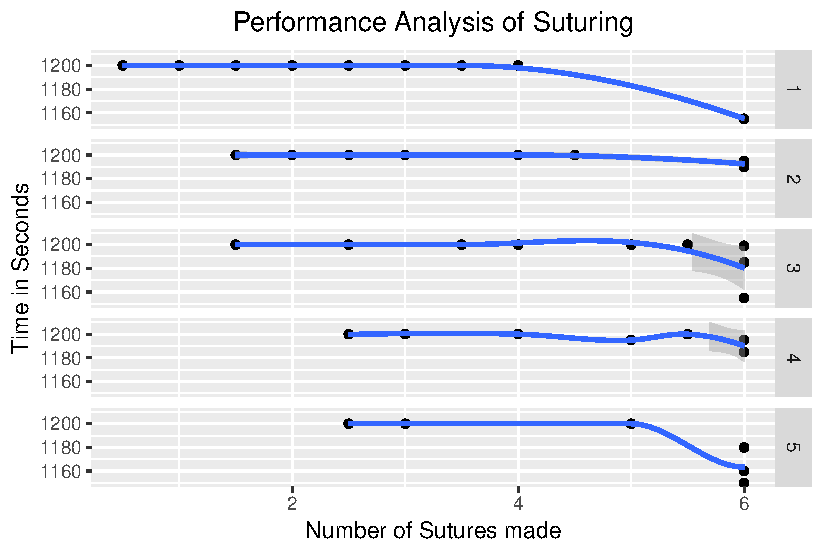
\includegraphics[width=0.5\textwidth]{SuturingVsTime.pdf}
	\caption{Performance Analysis of Suturing overTime }
	\centering
\end{figure}\\
From the figures, we understand that the number of sutures increases with each session. \\
To summarize it over all the subjects, we draw the bar plot with values of all subjects summed under each session , which gives us an understanding that with each session, the performance increases across all subjects.\\
When creating the linear model, and performing the analysis, we observe that the number of sutures is highly dependent on sessions .
Also, from the Performance analysis with respect to time plot, we infer that as the time decreases, the subjects are able to make more number of sutures and as number of session increases, the performance gets better.\\
\textbf{Inference}:\\
The number of sutures made increases with each session and takes less time, i.e the subjects are performing well.\\
\\
\FloatBarrier
\subsection*{4. Analysis of Scorers on Task:}
\addcontentsline{toc}{subsection} {Analysis of Scorers on Task}
\textbf{Hypothesis}:\\
$Null Hypothesis : H_0 = $ The mean of scores is same for both the Scorers\\
$Alternate Hypothesis : H_1 = $ The  mean of scores is different for both the Scorers\\
\\
\textbf{Assumptions}:\\
We perform shapiro.test to determine whether the Scores of Cutting and Suturing are normalized or not.We observe that the p-value is less than 0.05 in both the cases, which tells us that the columns are not normalized . Hence we perform Wilcoxon Test.\\
\textbf{Approach:Wilcox Test}:\\
\begin{figure}[!htb]
	\begin{minipage}[c]{0.5\linewidth}
	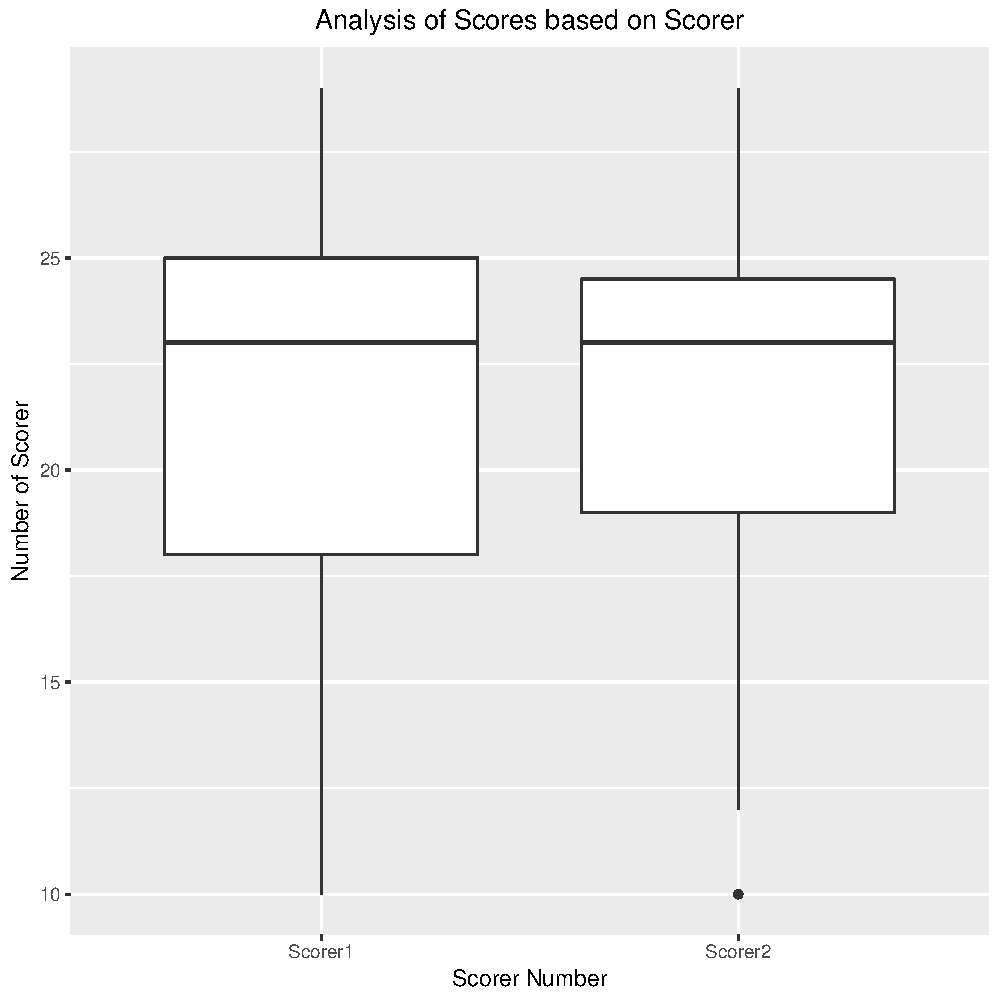
\includegraphics[width=\linewidth]{Cutting_ScorerVsScore.pdf}
	\caption{ Cutting Scores}
	\end{minipage}
	\hfill
	\begin{minipage}[c]{0.5\linewidth}
	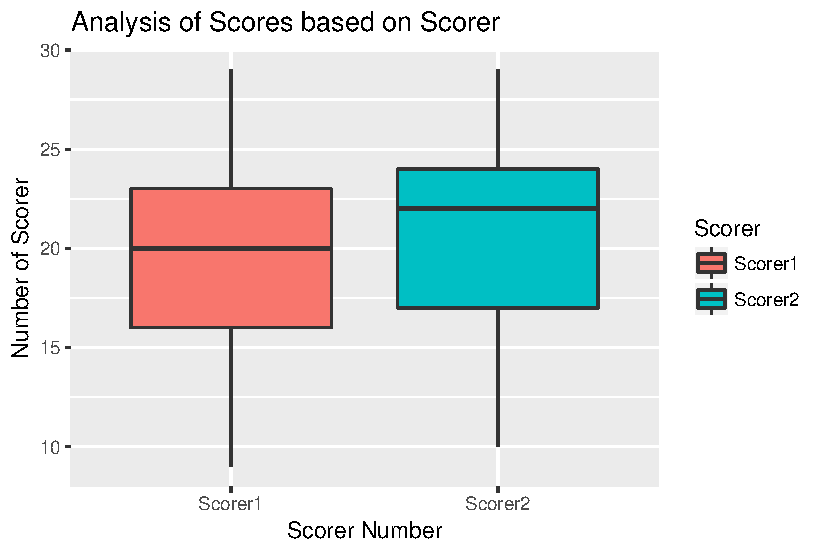
\includegraphics[width=\linewidth]{Suturing_ScorerVsScore.pdf}
	\caption{Suturing Scores}
	\end{minipage}
\end{figure}
\\
Cutting : When performed Wilcox test, p-value is 0.1676 which is greater than 0.05, which applies the means have not changed\\
Suturing: When performed Wilcox test, p-value is 0.00716, which less than 0.05, which states that the means of the scorers is different. \\
\\
\textbf{Inference}:\\
Scorer has impact on Suturing Task but not on Cutting Task,\\
\FloatBarrier
\subsection*{5. Analysis of Number of Sutures made with respect to sex and sessions:}
\addcontentsline{toc}{subsection} {Analysis of Number of Sutures made wrt. sex and sessions}
\textbf{Hypothesis}:\\
Null Hypothesis : $H_0 $= The number of sutures made is not significant on sex of the subject\\
Alternate Hypothesis : $H_1$ =  The number of sutures made is  significant on sex of the subject\\
\\
\begin{figure}[!htb]
	\centering
	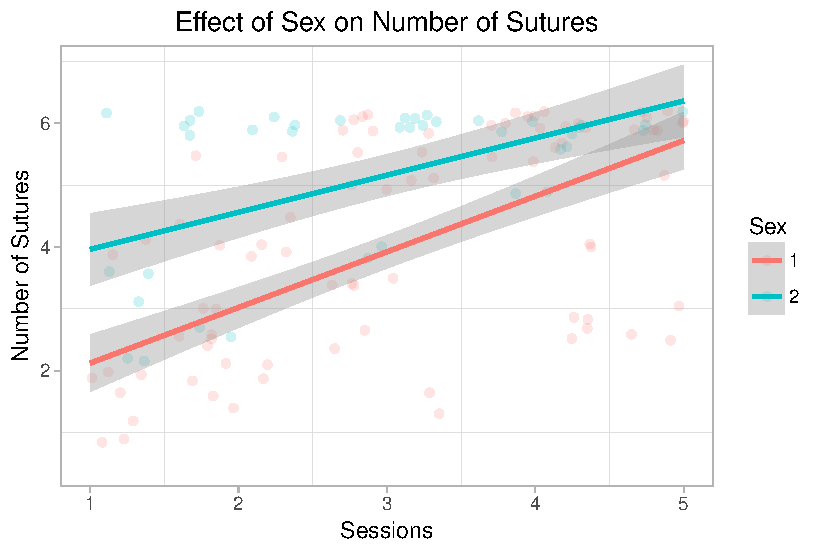
\includegraphics[width=0.5\textwidth]{SuturingVsSex.pdf}
	\caption{Interaction plot of Number of Sutures made wrt to Sex and Session}
	\centering
\end{figure}
\\
When performing the analysis for effect of Sutures on interaction of Sex and Sessions, we observe that, the p-value is 6.44e-11 which is way less than 0.05.\\
Also, from the interaction plot, we understand that the number of sutures made increases with the number of sessions and females make more number of sutures than males in average.\\
\\
\textbf{Inference}:\\
Sex has an effect on Number of Sutures made and females made more number of Sutures in 20 minutes and the number os sutures increases with each session, i.e subject's performance gets better with each session.\\
\FloatBarrier
\subsection*{6. Analysis of Performance With Respect to  TAI}
\addcontentsline{toc}{subsection}{Tai Score Effect on Performance}
\textbf{Assumptions}:\\
We perform shapiro.test to determine whether the Scores Below and Above Tai  are normalized or not.We observe that the p-value is less than 0.05 in both the cases, which tells us that the columns are not normalized . Hence we perform Wilcoxon Test.\\
\textbf{Hypothesis}:\\
Null Hypothesis : $H_0 = $ The performance score does not depend on tai score\\
Alternate Hypothesis : $H_1 = $ With increase in tai score, the performance score decreases\\
\\
\textbf{Approach:Wilxoxon Test}:
\begin{figure}[!htb]
	\begin{minipage}[c]{0.5\linewidth}
	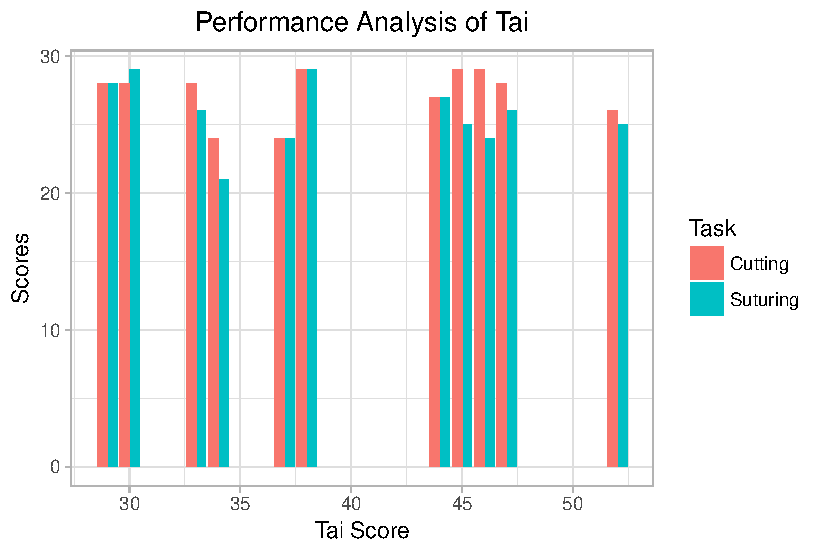
\includegraphics[width=\linewidth]{TaiVsScores.pdf}
	\caption{ Analysis of Tai Vs Scores}
	\end{minipage}
	\hfill
	\begin{minipage}[c]{0.5\linewidth}
	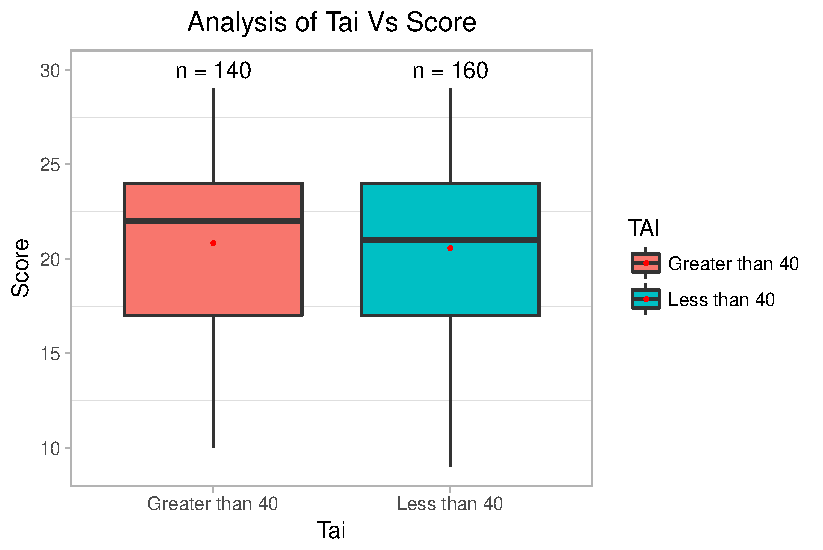
\includegraphics[width=\linewidth]{TaiVsScores_Box.pdf}
	\caption{Analysis of Tai Vs Scores}
	\end{minipage}
\end{figure}\\
Given, In the data, that Tai score above 40 means the subject is highly anxious. When performed T test, between all the values below or equal to 40 and above 40, we observe that the p-value is greater than 0.05, which indicates we accept the null hypothesis.\\
In addition, from the plots we can infer that the scores are pretty much the same, for both, above and below 40 Tai\\
\\
\textbf{Inference}:\\
With this, we infer that the in general, performance does not depend on how anxious the subject is and the tai score.
\FloatBarrier
\section*{Discussion}
\addcontentsline{toc}{section}{Discussion}
Further Research can be done 
\FloatBarrier
\section*{Conclusion}
\addcontentsline{toc}{section}{Conclusion}



%-------------------------------------------------------------------------------
% Appendix
%-------------------------------------------------------------------------------
\newpage
\section*{Appendix}
\addcontentsline{toc}{section}{Appendix}
\subsection*{List of Figures}
\addcontentsline{toc}{subsection}{List of Figures}
\subsection*{1. State Psychometric Data of all Subjects}
\begin{figure}[!htb]
	\centering
	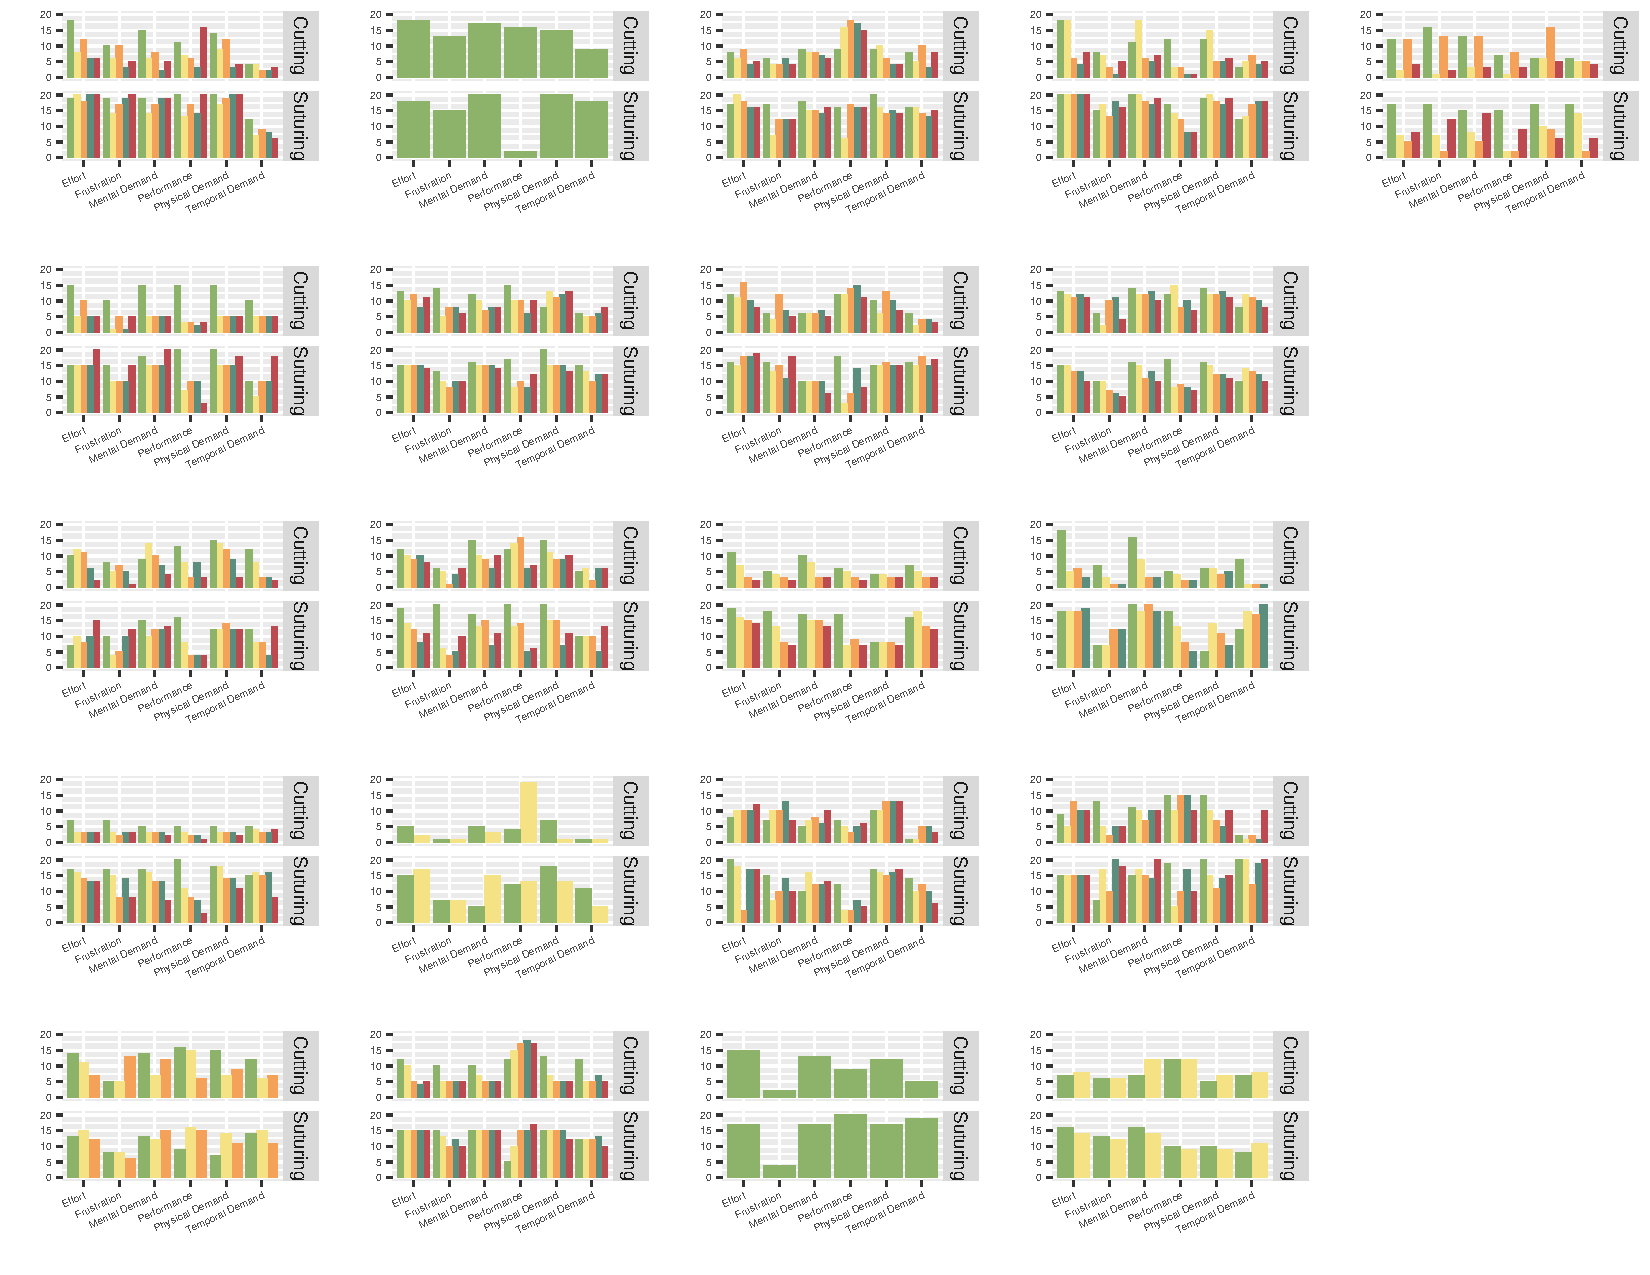
\includegraphics[width=1.0\textwidth]{multiplot_state_psycho.pdf}
	\caption{State Psychometric Data of all Subjects}
	\centering
\end{figure}
\FloatBarrier
\subsection*{2. Perinasal Perspiration (Stress) Signal Data of all subjects}
\begin{figure}[!htb]
	\centering
	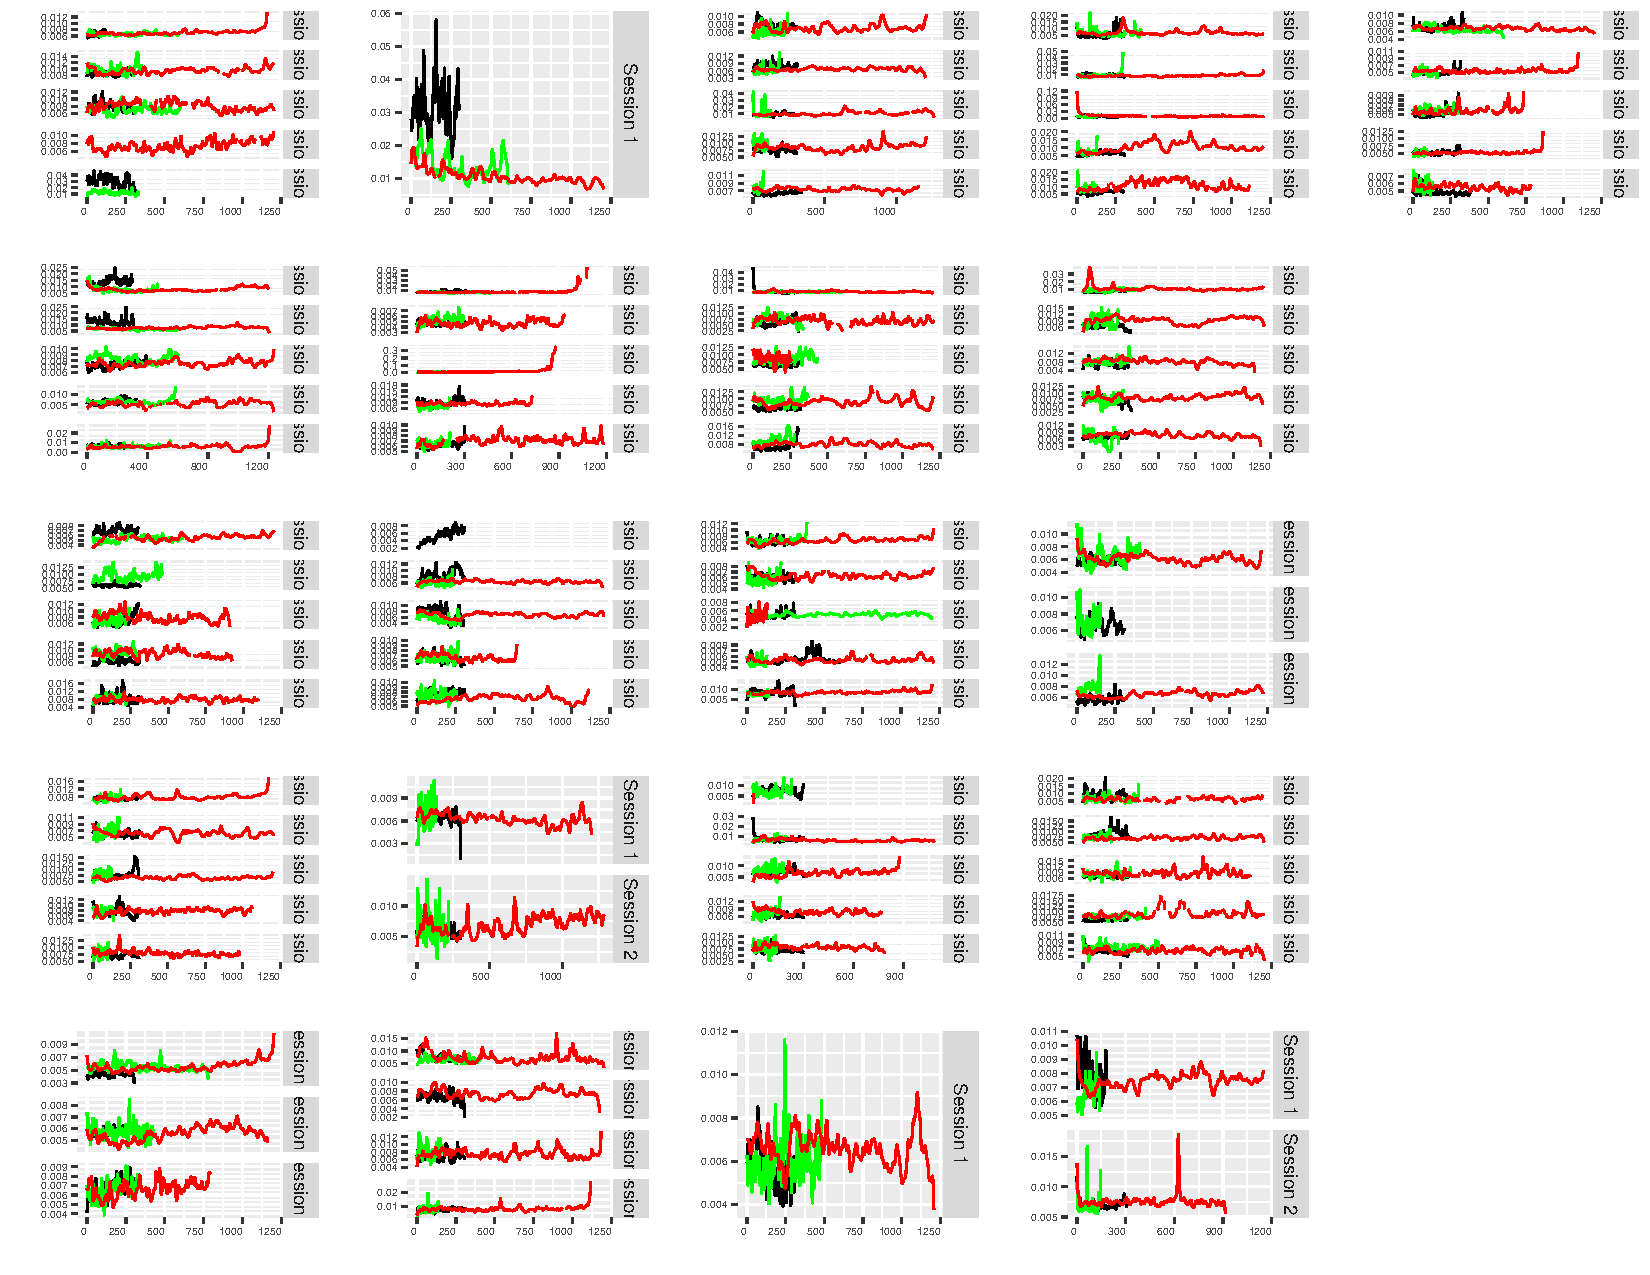
\includegraphics[width=1.0\textwidth]{multiplot_perinasal_percep.pdf}
	\caption{Perinasal Perspiration (Stress) Signal Data of all subjects}
	\centering
\end{figure}
\FloatBarrier
\subsection*{3. Suturing Time Performance of all Subjects}
\begin{figure}[!htb]
	\centering
	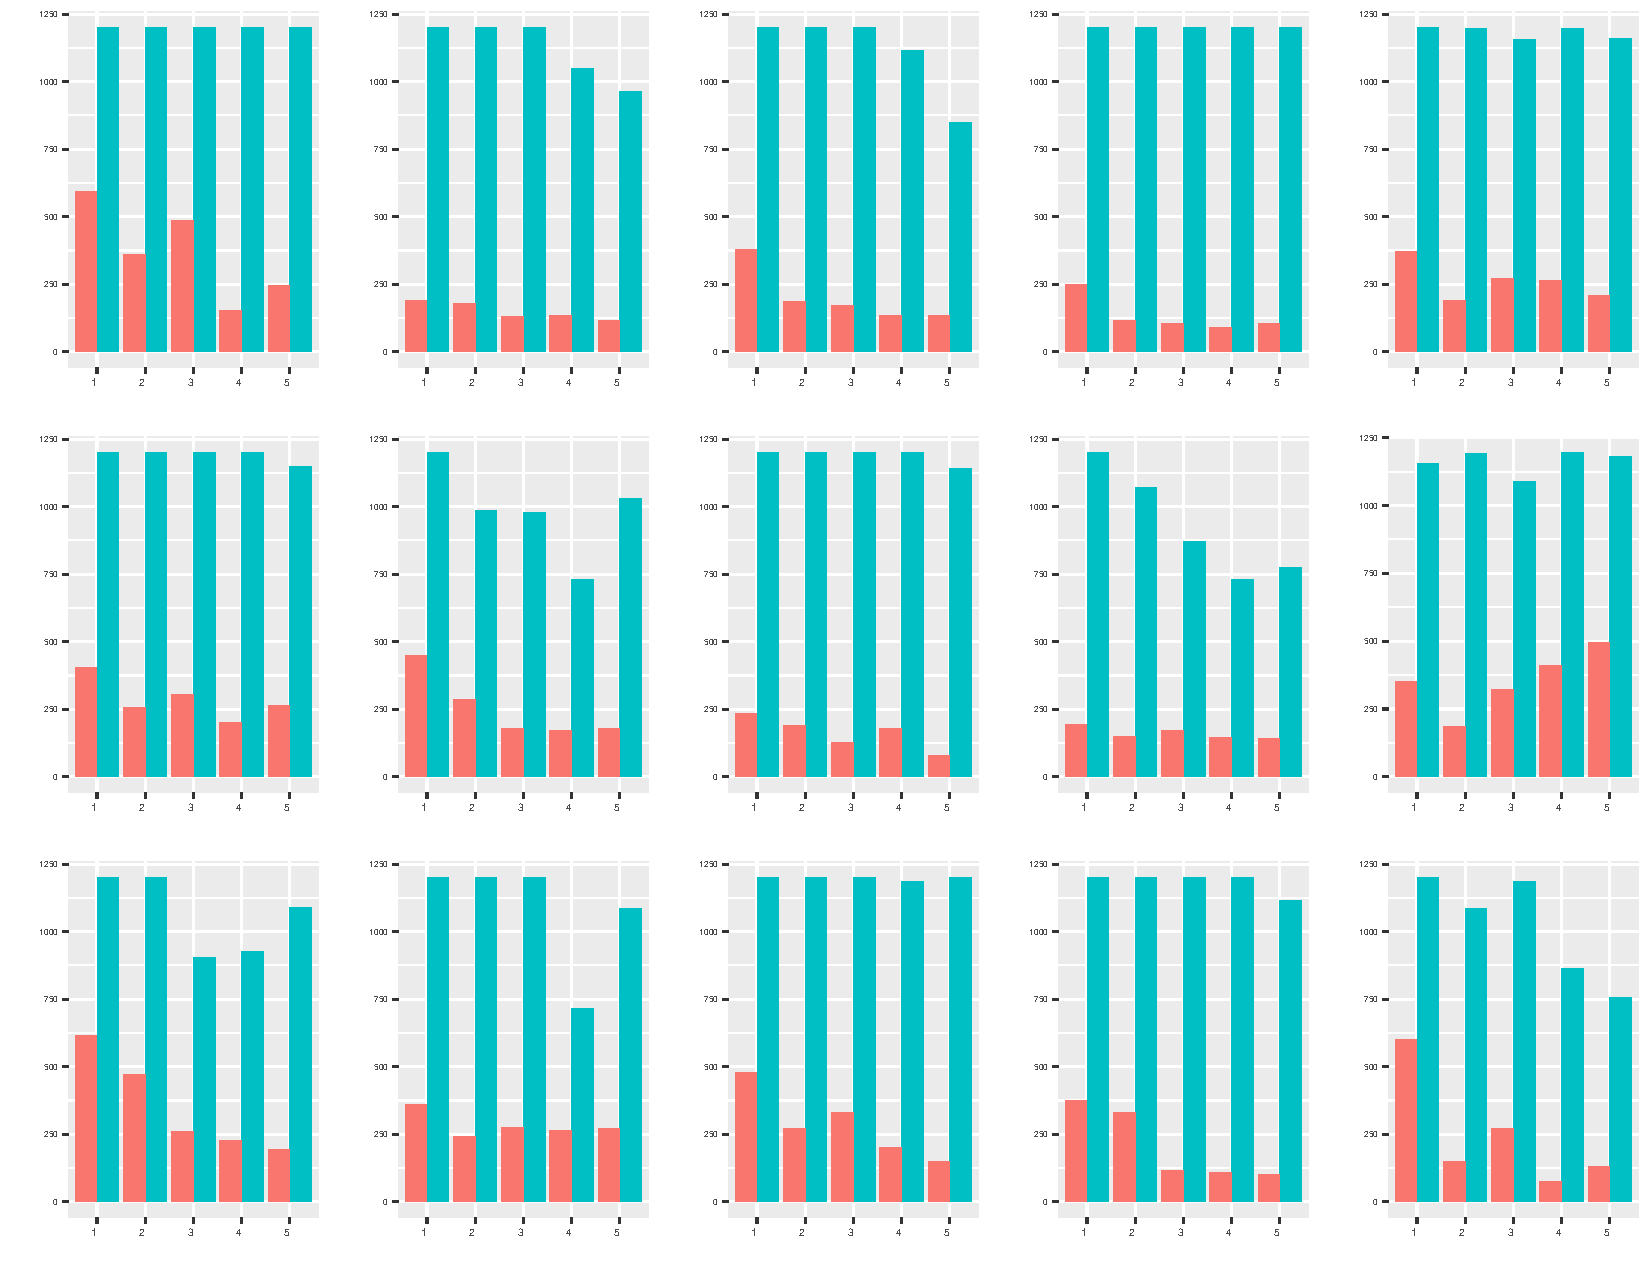
\includegraphics[width=1.0\textwidth]{multiplot_task_time.pdf}
	\caption{ Suturing Time Performance of all Subjects}
	\centering
\end{figure}
\FloatBarrier
\subsection*{4.Accuracy of Scores of all subjects}
\begin{figure}[!htb]
	\centering
	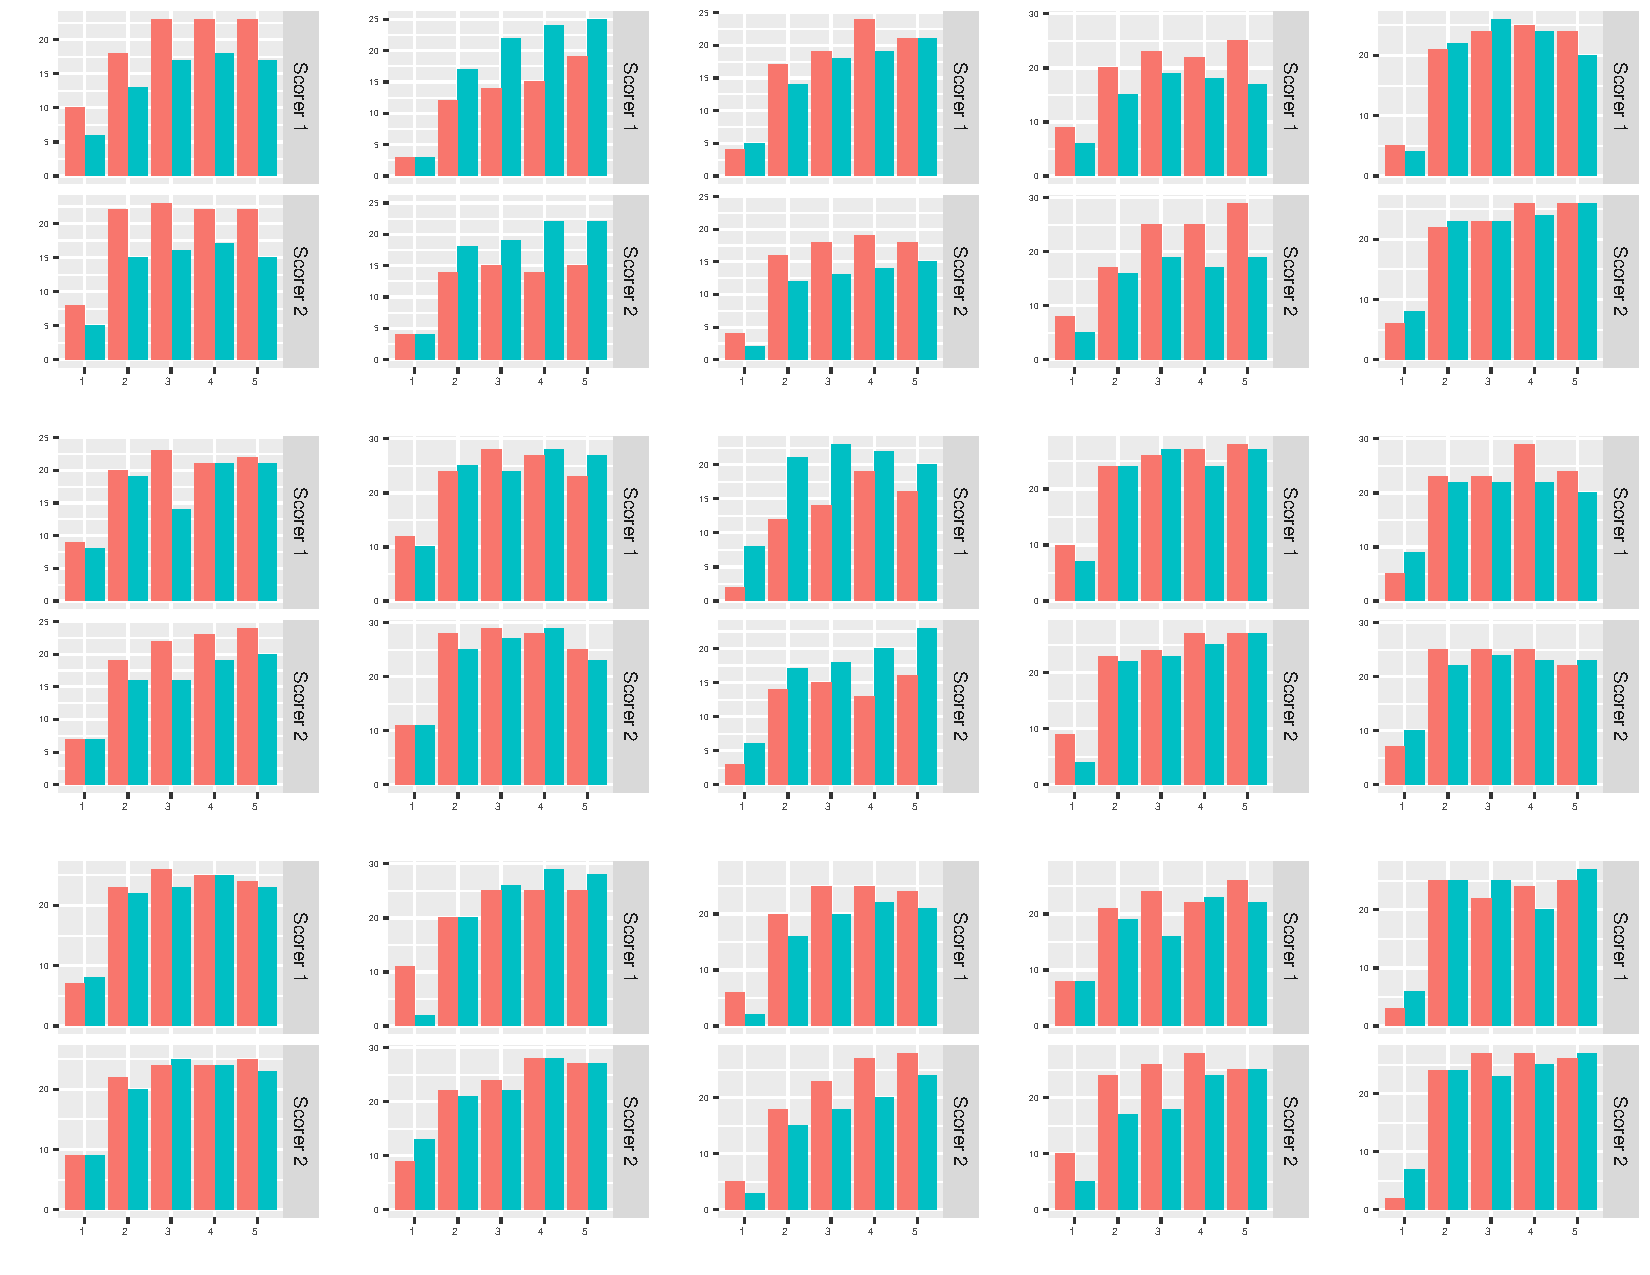
\includegraphics[width=1.0\textwidth]{multiplot_scorer.pdf}
	\caption{Accuracy of Scores of all subjects}
	\centering
\end{figure}
\FloatBarrier
\subsection*{5.Correlation Matrix Visualization of Plots of Data based on Task}
\begin{figure}[!htb]
	\centering
	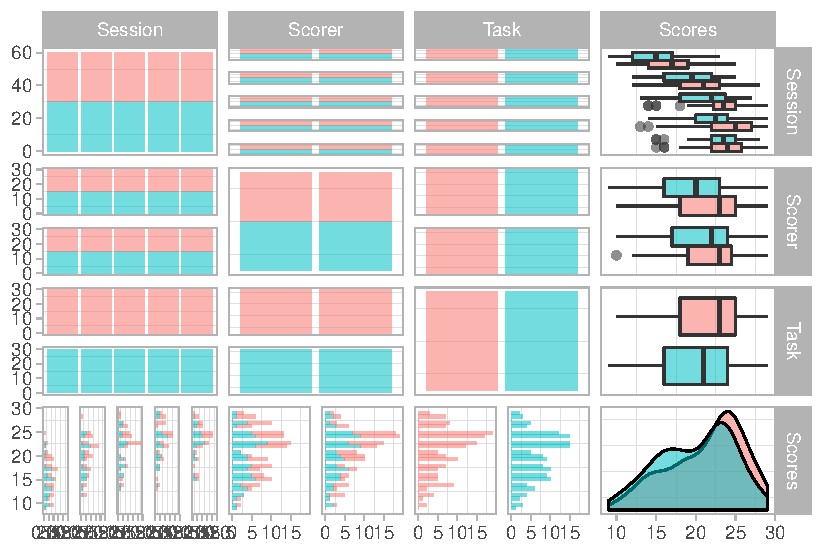
\includegraphics[width=1.0\textwidth]{Data_GGpairs.pdf}
	\caption{Accuracy of Scores of all subjects}
	\centering
\end{figure}
\FloatBarrier
\subsection*{6.Correlation Matrix Visualization of Plots of Cutting Data based on scorer}
\begin{figure}[!htb]
	\centering
	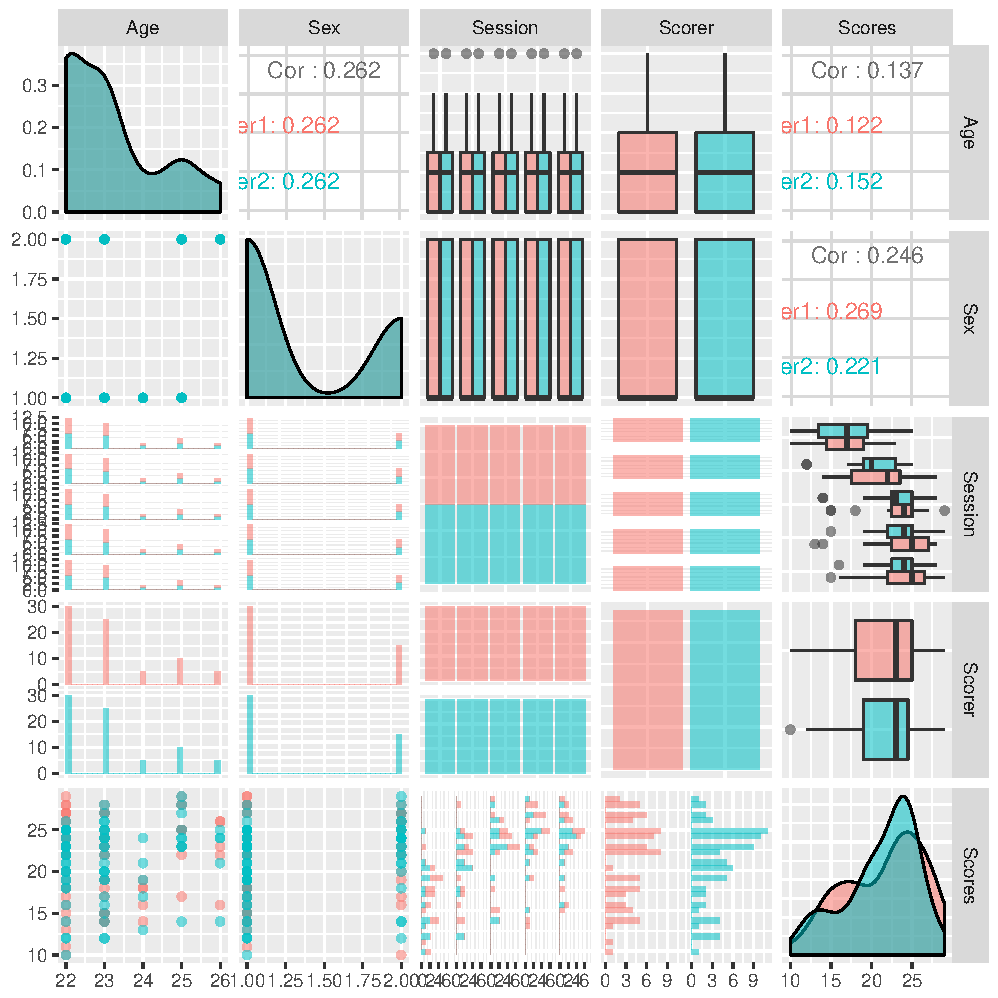
\includegraphics[width=1.0\textwidth]{Cutting_GGpairs.pdf}
	\caption{Accuracy of Scores of all subjects}
	\centering
\end{figure}
\FloatBarrier
\subsection*{7.Correlation Matrix Visualization of Plots of Suturing Data based on scorer}
\begin{figure}[!htb]
	\centering
	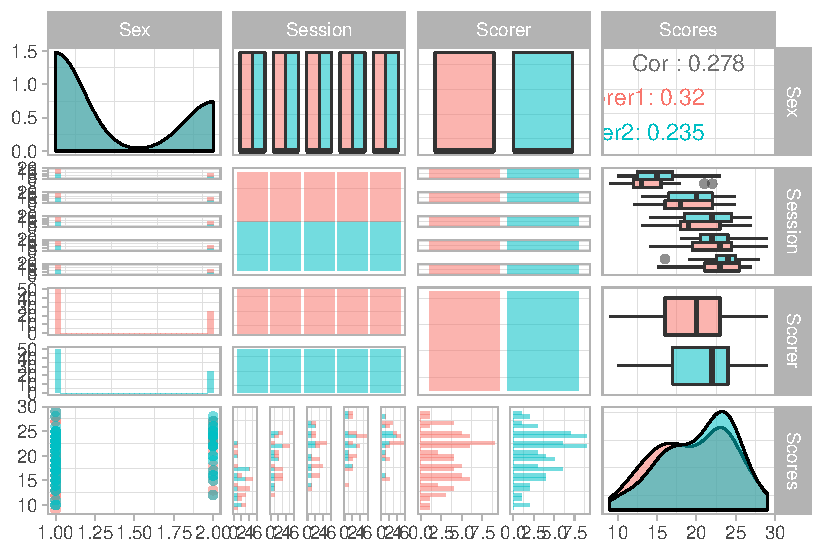
\includegraphics[width=1.0\textwidth]{Suturing_GGpairs.pdf}
	\caption{Accuracy of Scores of all subjects}
	\centering
\end{figure}

%-------------------------------------------------------------------------------
% REFERENCES
%-------------------------------------------------------------------------------
\newpage
\section*{References}
\addcontentsline{toc}{section}{References}




\end{document}

